%%
%% This is file `sample-manuscript.tex',
%% generated with the docstrip utility.
%%
%% The original source files were:
%%
%% samples.dtx  (with options: `all,proceedings,bibtex,manuscript')
%% 
%% IMPORTANT NOTICE:
%% 
%% For the copyright see the source file.
%% 
%% Any modified versions of this file must be renamed
%% with new filenames distinct from sample-manuscript.tex.
%% 
%% For distribution of the original source see the terms
%% for copying and modification in the file samples.dtx.
%% 
%% This generated file may be distributed as long as the
%% original source files, as listed above, are part of the
%% same distribution. (The sources need not necessarily be
%% in the same archive or directory.)
%%
%%
%% Commands for TeXCount
%TC:macro \cite [option:text,text]
%TC:macro \citep [option:text,text]
%TC:macro \citet [option:text,text]
%TC:envir table 0 1
%TC:envir table* 0 1
%TC:envir tabular [ignore] word
%TC:envir displaymath 0 word
%TC:envir math 0 word
%TC:envir comment 0 0
%%
%% The first command in your LaTeX source must be the \documentclass
%% command.
%%
%% For submission and review of your manuscript please change the
%% command to \documentclass[manuscript, screen, review]{acmart}.
%%
%% When submitting camera ready or to TAPS, please change the command
%% to \documentclass[sigconf]{acmart} or whichever template is required
%% for your publication.
%%
%%
%\documentclass[manuscript,screen,anonymous,review]{acmart}
\documentclass[manuscript,screen,review]{acmart}

\usepackage{enumitem}
\usepackage{csquotes}

\usepackage{tabularray}
\usepackage{tabularx}
\usepackage{multirow, makecell}
\usepackage{tabularx,array,booktabs}
\usepackage{array}
\usepackage{subcaption}
\usepackage{footnote}
\usepackage[commandnameprefix=always, draft]{changes}
\usepackage{multicol}
\makeatletter
\AddToHook{cmd/added/before}{\def\Changes@AuthorColor{blue}}
\AddToHook{cmd/deleted/before}{\def\Changes@AuthorColor{red}}
\AddToHook{cmd/replaced/before}{\def\Changes@AuthorColor{cyan}}
\makeatother

\newcolumntype{P}[1]{>{\centering\arraybackslash}p{#1}}
\newcommand{\specialcell}[2][b]{\begin{tabular}[#1]{@{}c@{}}#2\end{tabular}}

\usepackage{tikz}
\usetikzlibrary{automata, positioning, arrows, shapes.geometric,calc, shapes.multipart}

%%
%% \BibTeX command to typeset BibTeX logo in the docs
\AtBeginDocument{%
  \providecommand\BibTeX{{%
    Bib\TeX}}}

%% Rights management information.  This information is sent to you
%% when you complete the rights form.  These commands have SAMPLE
%% values in them; it is your responsibility as an author to replace
%% the commands and values with those provided to you when you
%% complete the rights form.
\setcopyright{acmlicensed}
\copyrightyear{2025}
\acmYear{2025}
\acmDOI{XXXXXXX.XXXXXXX}
%% These commands are for a PROCEEDINGS abstract or paper.
\acmConference[Conference acronym 'XX]{Make sure to enter the correct
  conference title from your rights confirmation email}{June 03--05,
  2018}{Woodstock, NY}
%%
%%  Uncomment \acmBooktitle if the title of the proceedings is different
%%  from ``Proceedings of ...''!
%%
%%\acmBooktitle{Woodstock '18: ACM Symposium on Neural Gaze Detection,
%%  June 03--05, 2018, Woodstock, NY}
\acmISBN{978-1-4503-XXXX-X/2018/06}


%%
%% Submission ID.
%% Use this when submitting an article to a sponsored event. You'll
%% receive a unique submission ID from the organizers
%% of the event, and this ID should be used as the parameter to this command.
%%\acmSubmissionID{123-A56-BU3}

%%
%% For managing citations, it is recommended to use bibliography
%% files in BibTeX format.
%%
%% You can then either use BibTeX with the ACM-Reference-Format style,
%% or BibLaTeX with the acmnumeric or acmauthoryear sytles, that include
%% support for advanced citation of software artefact from the
%% biblatex-software package, also separately available on CTAN.
%%
%% Look at the sample-*-biblatex.tex files for templates showcasing
%% the biblatex styles.
%%

%%
%% The majority of ACM publications use numbered citations and
%% references.  The command \citestyle{authoryear} switches to the
%% "author year" style.
%%
%% If you are preparing content for an event
%% sponsored by ACM SIGGRAPH, you must use the "author year" style of
%% citations and references.
%% Uncommenting
%% the next command will enable that style.
%%\citestyle{acmauthoryear}


%%
%% end of the preamble, start of the body of the document source.
\begin{document}

%%
%% The "title" command has an optional parameter,
%% allowing the author to define a "short title" to be used in page headers.
\title{Towards a Visual FactSheet}

%%
%% The "author" command and its associated commands are used to define
%% the authors and their affiliations.
%% Of note is the shared affiliation of the first two authors, and the
%% "authornote" and "authornotemark" commands
%% used to denote shared contribution to the research.

\author{SM Mozammal Hossain}
\affiliation{
	\institution{University of New Brunswick}
	\streetaddress{550 Windsor Street}
	\city{Fredericton}
	\state{NB}
	\country{Canada}
	\postcode{E3B 5A3}
}
\email{mozammal.hossain@unb.ca}

\author{Kenneth B. Kent}
\affiliation{
	\institution{University of New Brunswick}
	\streetaddress{550 Windsor Street}
	\city{Fredericton}
	\state{NB}
	\country{Canada}
	\postcode{E3B 5A3}
}
\email{ken@unb.ca}

\author{Phil Munz}
\affiliation{
	\institution{TrojAI}
	\streetaddress{14 King St., Suite 102}
	\city{Saint John}
	\state{NB}
	\country{Canada}
	\postcode{E2L 1G2}
}
\email{phil.munz@troj.ai}

%%
%% By default, the full list of authors will be used in the page
%% headers. Often, this list is too long, and will overlap
%% other information printed in the page headers. This command allows
%% the author to define a more concise list
%% of authors' names for this purpose.
\renewcommand{\shortauthors}{mozammal et al.}

%%
%% The abstract is a short summary of the work to be presented in the
%% article.
\begin{abstract}
%  Machine Learning (ML) model development is moving at a breakneck speed and becoming a common term due to the numerous prominent and promising information technology companies applying Generative Artificial Intelligent (GAI) technology in many of their publicly available artificially intelligent services (AIS). While AIS became very popular too quickly among general users, little or no information is publicly available about how the underlying ML models were developed, trained, and what training datasets were used. There is also inadequate information about how trustworthiness, transparency, and fairness were achieved, which are the main pillars of Artificial Intelligence Governance. Most users who use publicly available AIS are poorly informed through the terms and conditions about what they are paying (although they are marketed as free) for receiving free services. \chadded{We argue that user were not properly informed how users and companies are mutually benefit from using those services}. We believe all publicly available AIS must inform users clearly about the mutual benefit of using the service. In this paper, we are proposing a framework, i.e., Visual FactSheet (VFS) intended for AIS. The framework is designed with end users in mind. Its primary objective is to visually depict one or many properties of free AIS so that users can make informed decisions before using it. Furthermore, we propose formal definitions intended for various FactSheet users. We believe our proposed definitions will guide and help generate an effective FactSheet.
  
  The development of machine learning (ML) models is advancing rapidly and has become a widely recognized concept, largely due to leading technology companies integrating generative artificial intelligence (GAI) into many of their publicly accessible artificially intelligent services (AIS). Although AIS has gained popularity at an unprecedented pace among general users, there is limited public information about how these ML models are built, trained, and what datasets are utilized. Additionally, details on achieving trustworthiness, transparency, and fairness—key principles of AI governance—are scarce. Most users of free AIS services remain poorly informed through terms and conditions about what they are actually paying for, despite these services being marketed as free. We contend that users have not been adequately informed about the mutual benefits for both users and companies. Therefore, we argue that all publicly available AIS can clearly communicate these mutual benefits. In this paper, we introduce a framework called Visual FactSheet (VFS) for AIS, designed with end users in mind. Its main goal is to visually present one or more attributes of free AIS, enabling users to make informed choices before engaging with them. Furthermore, we propose formal definitions tailored for different FactSheet stakeholders, which we believe will assist in creating effective and meaningful FactSheets.
  
\end{abstract}

%%
%% The code below is generated by the tool at http://dl.acm.org/ccs.cfm.
%% Please copy and paste the code instead of the example below.
%%
\begin{CCSXML}
<ccs2012>
 <concept>
  <concept_id>00000000.0000000.0000000</concept_id>
  <concept_desc>Do Not Use This Code, Generate the Correct Terms for Your Paper</concept_desc>
  <concept_significance>500</concept_significance>
 </concept>
 <concept>
  <concept_id>00000000.00000000.00000000</concept_id>
  <concept_desc>Do Not Use This Code, Generate the Correct Terms for Your Paper</concept_desc>
  <concept_significance>300</concept_significance>
 </concept>
 <concept>
  <concept_id>00000000.00000000.00000000</concept_id>
  <concept_desc>Do Not Use This Code, Generate the Correct Terms for Your Paper</concept_desc>
  <concept_significance>100</concept_significance>
 </concept>
 <concept>
  <concept_id>00000000.00000000.00000000</concept_id>
  <concept_desc>Do Not Use This Code, Generate the Correct Terms for Your Paper</concept_desc>
  <concept_significance>100</concept_significance>
 </concept>
</ccs2012>
\end{CCSXML}

\ccsdesc[500]{Do Not Use This Code~Generate the Correct Terms for Your Paper}
\ccsdesc[300]{Do Not Use This Code~Generate the Correct Terms for Your Paper}
\ccsdesc{Do Not Use This Code~Generate the Correct Terms for Your Paper}
\ccsdesc[100]{Do Not Use This Code~Generate the Correct Terms for Your Paper}

%%
%% Keywords. The author(s) should pick words that accurately describe
%% the work being presented. Separate the keywords with commas.
\keywords{Do, Not, Use, This, Code, Put, the, Correct, Terms, for,
  Your, Paper}

\received{20 February 2007}
\received[revised]{12 March 2009}
\received[accepted]{5 June 2009}

%%
%% This command processes the author and affiliation and title
%% information and builds the first part of the formatted document.
\maketitle

\section{Introduction}\label{intro}
	
	AIS have become increasingly integrated into our daily lives. Although ML has been a prominent research area for years, it struggled to establish its superiority solving problems that are commercially viable. This led to slower adoption of ML technology. Limitations in ML algorithms, tools, hardware resources, and availability of training data contributed to this lower commercial adoption. Over the past decade, ML has evolved dramatically and became a core component of many automated services, e.g., answering citizen inquiries about unemployment benefits, welfare programs, and many more \cite{10.1093/ppmgov/gvaf013}. Extensive research has led to the development of numerous ML strategies, techniques, and algorithms. With advancements in Deep Learning (DL), Natural Language Processing (NLP), and most recently Large Language Models (LLMs), ML has proven its ability to tackle complex problems having commercial value \cite{li_impact_2023} \cite{pugliese_machine_2021}. As a result, leading corporations such as Microsoft, Google, IBM, Amazon etc. began investing heavily to integrate ML into their products. Although Google and Amazon experimented and incorporated ML techniques in their products since 2014 in limited scope, after observing DL and LLM's recent achievements in image detection and language processing, both companies commercially engage this technology to improve their search results and product recommendations. Other influential players, e.g., IBM, Meta, and many more are also adopting ML technology. Today, it is hard to find companies, ranging from mid size to large, have a product offering without having ML capability.
	
	ML requires a large amount of data for its training. Both leading and promising companies interested in developing ML based services or applications have been collecting data, actively or passively, for a long time. By offering free services such as search engines, social media, e-commerce platform, etc., companies collect data. Loyalty programs is another technique retail companies applies to collect consumer data. The intention is that these companies will use those for user profiling and provide curated product recommendation or targeted advertisement. The process of data collection still continues today. At present, 19.8 billion IOT devices are \cite{statistica_2} connected to internet generating 2.5 quintillion bytes daily \cite{seedscientific}. This growth is projected to be continue and by 2034 40.6 billion IOT device will be connected and by 2029 will produce 527.5 zettabytes  of data annually \cite{statistica_1} \cite{statistica_2}.
	
	Until the introduction of General Data Protection Regulation (GDPR) in 2016, companies enjoyed an extended period without answering to any regulatory authority about how they are collecting data and what is their intention to use them \cite{GDPR2016a}. Same applies to ML model development until the emergence of AI governance policy. GDPR, introduced by the European Union (EU), enforces very strict guidelines for collecting, processing, protecting, ownership, retention period, and use of data for any purpose. This poses an enormous data collection and usage challenge for companies who either a developer or user of information technology. ML model development was not free from challenges as well. 
	
	As GDPR became effective in May 2018 for all EU member countries. This enforcement created an enormous challenge for companies involved in ML model development. However they all adapted to this challenge and to comply with GDPR regulations added clauses for data collection in their \enquote{Terms and Conditions} or \enquote{Terms of use} agreement (a legal contract between the service provider and users in text form) which traditionally used for safeguarding product and its usage \cite{buttarelli_we_2019}. A similar text based approach is also being proposed but yet to applied widely for achieving ML model's fairness of making recommendation and ability to explain. Since EU AI act is expected to take effect except one article on August 2nd, 2026, companies are still enjoying this freedom. 
	
	\textbf{License or terms of conditions are buried very deep, it hard to find right information easily. Require good navigation skills}
	
	For AIS services, there are limited public information about how underlying ML models were built, trained, and what datasets were used for training. Hence, they frequently criticized for their lack of transparency, commonly referred to as the ‘black box’ problem, where the reasoning behind its decisions or recommendations remains unclear \cite{app15020672} \cite{10.2478} \cite{JSSv036i11}. Since AIS is gradually becoming an integral part of non-technical or general people's daily activity, we believe there is a need for user friendly documentation framework intended for the general population, a user who has basic level of competency in understanding and using digital tools \cite{literacy}
	
%	In the paper, we are proposing a visual documentation framework for multiple user groups capturing all necessary and critical information of an AI model or AIS to achieve trustworthiness. We believe our proposed framework is superior and an extended version of other similar efforts. Until now, such documentation frameworks were intended for highly technical personnel who possess sufficient technological background, education, and skills to interpret the outcome from the document. Since AIS is gradually becoming an integral part of non-technical or general people's daily activity, we believe there is a need for a user friendly documentation framework intended for the general population, a user who has basic level of competency in understanding and using digital tools \cite{literacy}.
	
	
%	ML model development is advancing rapidly. Driven by leading technology companies, it has become a widely recognized technique used into many publicly available AI services (AIS). Although AIS has quickly gained popularity among general users, there is limited public information regarding how companies built their ML models, trained, and what datasets were used. Furthermore, details on achieving trustworthiness, transparency, and fairness, key principles of AI governance, remain scarce. Most users of these services receive minimal clarity through terms and conditions about what they are exchanging for free access.

%	DL and LLM ML techniques require a large amount of data for training purposes. Using synthetic data, researchers were able to showcase the excellence of the mentioned ML techniques in a controlled environment but were not always able to convince information technology companies to adapt those, although all parties agreed that the technology has tremendous potential \cite{eastwood_study_2023} \cite{house_executive_2022}. With the advancement and extensive use of the internet, gradually data became abundantly available to many well established large corporations. Many of them did not know what to do with those data or could not process those for future benefit. However, the amount of data generation or production was growing exponentially. It is predicted that by 2025, 100+ zettabytes of data will be produced each year \cite{vuleta_how_2021}. To make use of the large amount of data, ML became the most suitable and applicable technology. Well established corporations, e.g., Microsoft, Google, IBM, and Amazon, started to invest their resources heavily with the intention to apply ML technology into their products. Google started using NLP techniques in their search engine in 2015 \cite{schwartz_how_2022}. In a similar fashion, Amazon started their work on this domain in 2014 to make their e-commerce platform more efficient \cite{levy_how_2018}. Both companies wanted to provide better search results or product recommendations. IBM also joined this race by introducing their Watson offering with the intention that it will become a platform for ML application development, deployment, and monitoring \cite{ibm_ibm_nodate}. Microsoft invested in developing LLM with the intention of providing chatbot-type services \cite{cambon_early_2023}. At present, the companies mentioned above, and many promising new ones are focusing on bringing GAI into many of their products.
	
%	Deep Learning (DL) and Large Language Model (LLM) techniques require substantial amounts of data for effective training. Researchers initially relied on synthetic datasets to demonstrate the capabilities of these methods in controlled environments. However, despite recognizing their immense potential, technology companies were not always persuaded to adopt them. With the widespread growth of the internet, data gradually became abundant for many large, established corporations. Initially, these organizations struggled to utilize or process the data for future benefits, even as data generation continued to grow exponentially. By 2025, global data production is projected to exceed 100 zettabytes annually. Mac


%	Machine Learning (ML) emerged as the most practical solution for leveraging this massive data volume. Leading corporations such as Microsoft, Google, IBM, and Amazon began investing heavily to integrate ML into their products. For example, Google incorporated Natural Language Processing (NLP) into its search engine in 2015, while Amazon started applying ML in 2014 to enhance its e-commerce platform. Both aimed to improve search results and product recommendations. IBM entered the field with its Watson platform, designed for ML application development, deployment, and monitoring, while Microsoft focused on developing LLMs for chatbot services. Today, these companies, along with emerging players, are working to embed Generative AI (GAI) into a wide range of products.
	
	

%\section{Problem Statement}

%Until the introduction of General Data Protection Regulation (GDPR) in 2016, which became effective in May 2018, by the European Parliament and Council of the European Union, companies had little or no concern for informing users or consumers about rights, responsibilities, and ownership of those collected data and their usage \cite{GDPR2016a} \cite{rossow_birth_2018}. This regulation enforces very strict guidelines for collecting, processing, protecting, ownership, retention period and use of data for any purpose. This poses an enormous challenge for companies involved in ML model development. However they all adapted to this challenge and maintained their data collection process by adding a few clauses for data collection and uses in their \enquote{Terms and Conditions} or \enquote{Terms of use} agreement (a legal contract between the service provider and users), before signing. Companies use this not only to protect their product but also to overcome GDPR regulations \cite{buttarelli_we_2019}.

%The development of ML models is progressing rapidly, especially as leading technology companies increasingly integrate Generative Artificial Intelligence (GAI) into their publicly accessible AIS. Although AIS has quickly gained popularity among its users, there are limited public information about how these underlying ML models were built, trained, and what datasets were used for training purposes. Hence, ML is frequently criticized for its lack of transparency, commonly referred to as the ‘black box’ problem, where the reasoning behind its decisions or recommendations remains unclear \cite{app15020672} \cite{10.2478} \cite{JSSv036i11}. As countries introduce AI regulatory policies, ensuring transparency through explainability has become a mandatory requirement for ML assisted software services. Most users engaging with free AIS are only superficially informed through terms and conditions, leaving them unaware of what data they are truly exchanging for access to these free services. We argue that users are not sufficiently educated about the mutual benefits involved in using AIS. Therefore, we advocate for clearer communication between AIS providers and users.

%	The development of ML models is progressing rapidly, especially as leading technology companies increasingly integrate Generative Artificial Intelligence (GAI) into their publicly accessible AIS. Although AIS has quickly gained popularity among its users, there are limited public information about how these underlying ML models were built, trained, and what datasets were used for training purposes. Hence, ML is frequently criticized for its lack of transparency, commonly referred to as the ‘black box’ problem, where the reasoning behind its decisions or recommendations remains unclear \cite{app15020672} \cite{10.2478} \cite{JSSv036i11}. As countries introduce AI regulatory policies, ensuring transparency through explainability has become a mandatory requirement for ML assisted software services. Most users engaging with free AIS are only superficially informed through terms and conditions, leaving them unaware of what data they are truly exchanging for access to these free services. We argue that users are not sufficiently educated about the mutual benefits involved in using AIS. Therefore, we advocate for clearer communication between AIS providers and users.
	
%	There is a growing concern about fairness, accountability, and transparency of the ML models along with inexplicability of the decisions these AISs are making. Black box models can be vulnerable for adversarial attacks and be used in a hazardous manner \cite{house_executive_2023}. For example, irresponsible use of ML or a compromised model due to an adversarial attack could cause disinformation, discrimination, cyber fraud, automatic harmful cyber-attack on critical infrastructure and even pose risks to national security \cite{house_executive_2023}. The biggest concern for any AI application is, whether it is making ethical fair decisions. A strong oversight must be placed during development, deployment, and maintenance or model service phase making sure it is operating in an ethical manner. In other words, it must be able to explain and provide reasoning for a decision. So, there is an immediate need for a set of artificial intelligence governance (AIG) tools for identifying possible fairness, accountability, transparency issues and make those models trustworthy.

%\section{Motivation}\label{motivation}

%	The term \enquote{AI}, i.e., artificial intelligence, has exceeded its boundaries from the scientific community, computer scientists and became a common terminology among the general population and so have Data Science and Machine Learning \cite{arya_ai_2022}. Thanks to Google, Microsoft, and OpenAI for their publicly available large language models, ChatGPT and Gemini are making their marks and making life-style changes to common people everyday \cite{openai2025chatgpt} \cite{geminiteam2024}. These are only a few applications that are changing people's life-styles. Grammerly, an AI-powered writing assistant, is gradually \chadded{increasing} its popularity among students, professionals, researchers and many more. While large language model (LLM) based ChatGPT, and Gemini act as chatbots and can do many things, Grammerly focused on one problem, i.e., how to improve one's writing or generate a template for a specific use.
	
	
%	Artificial intelligence (AI) has moved beyond the confines of the scientific community and computer science, becoming a widely recognized term among the general public—alongside Data Science and Machine Learning \cite{arya_ai_2022}. Thanks to companies like Google, Microsoft, and OpenAI, large language models such as ChatGPT and Gemini are now publicly accessible, influencing everyday life and driving lifestyle changes \cite{openai2025chatgpt} \cite{geminiteam2024}. These represent just a few examples of applications transforming how people live and work. Grammarly, an AI-powered writing assistant, continues to gain popularity among students, professionals, and researchers. While LLM-based tools, e.g. ChatGPT and Gemini function as versatile chatbots capable of performing numerous tasks, Grammarly focuses on a specific challenge: improving writing quality and generating templates for targeted purposes.
		

%	For a long time, the general population was unaware of the use of AI technology in many products or services they use in their day-to-day life. Search engines, e.g., Google, became an integral part for our everyday life. Google started using AI technology in their search engine have been using since 2015 for providing better results. Over time they added new AI technologies to the search engine, e.g., RankBrain, and Neural matching was added in 2015 and 2018 respectively \cite{schwartz_how_2022}. It is fair to say adding these technologies in the search engine were not discussed much publicly and very few people outside the information technology domain were aware of this development. The same is true for Amazon, Meta (formerly Facebook), IBM, and Microsoft to name a few \cite{levy_how_2018} \cite{ibm_ibm_nodate} \cite{cambon_early_2023} \cite{dunn_introducing_2016}. Amazon started its planning for use of AI technology in 2014 to provide better product search for their customers \cite{levy_how_2018}. It is again fair to say, the general population were unaware of the technological advancements and happily enjoyed the improved service. With the first release of ChapGPT by OpenAI in November 2022, the general population suddenly realized the enormous capability of AI technologies.

%	The Machine Learning model requires a large amount of data for its training. Both prominent and promising information technology companies interested in developing ML-based services or applications have been collecting required training data actively or passively for a long time. Search engines, social media, and e-commerce platform companies collect data when one uses their free services. Loyalty programs launched by many retail companies are also a well-established mechanism developed for collecting user or consumer data. One of the use cases for collecting such data is for developing/updating their ML model for user profiling, product recommendation or developing new technologies. Until the introduction of General Data Protection Regulation (GDPR) in 2016, which became effective in May 2018, by the European Parliament and Council of the European Union, companies had little or no concern for informing users or consumers about rights, responsibilities, and ownership of those collected data and their usage \cite{GDPR2016a} \cite{rossow_birth_2018}. This regulation enforces very strict guidelines for collecting, processing, protecting, ownership, retention period and use of data for any purpose. This poses an enormous challenge for companies involved in ML model development. However they all adapted to this challenge and maintained their data collection process by adding a few clauses for data collection and uses in their \enquote{Terms and Conditions} or \enquote{Terms of use} agreement (a legal contract between the service provider and users), before signing. Companies use this not only to protect their product but also to overcome GDPR regulations \cite{buttarelli_we_2019}.
	
%	For English speaking adults, the average oral reading rate is 183 words per minute (wpm) and the silent reading rate can be up to 280-320 wpm \cite{obar_biggest_2016}\cite{brysbaert_how_2019}. Table \ref{tab:lincenseLength} shows the word count of a license agreements for some of the most popular and widely used applications or services. It is surprising to observe that some of the most popular free service providers, i.e., Facebook, Tinder, Microsoft, etc., crafted their license agreements in such a way that for a regular user it could take 14.4 to 63.5 minutes to read. Table \ref{tab:lincenseLength} results were based on 2020 data. We assume that most of the users did not spend much time to review and understand their rights, responsibilities, data collection, and possible usage before agreeing to it. \chadded{Our assumption is based on the survey findings conducted by Obar et al. where participants agreed to share their data with NSA, employer, and providing a first-born child as payment for social networking service (SNS) access \cite{obar_biggest_2016}. }We believe companies must inform its users about their obligation before using their services especially data collection, retention, and processing for AI based services.
%	
%	\begin{table}
%		\begin{tabular}{|l|c|c|l|c|c|}
%			\hline
%			\specialcell{Application or\\ Service} & \specialcell{Word\\Count} & 
%			\specialcell{How many minutes \\to read? (240 wpm)} & \specialcell{Application or\\ Service} & 
%			\specialcell{Word\\Count} & \specialcell{How many minutes \\to read? (240 wpm)}\\
%			\midrule
%			Microsoft & 15,260 & 63.5 & Spotify & 8,600 & 35.8\\
%			\hline
%			Apple (Media Services) & 7,314 & 30.5 & Zoom & 6,891 & 28.7\\
%			\hline
%			Tinder & 6,215 & 25.9 & Uber & 5,658 & 23.6\\
%			\hline
%			Bumble & 5,442 & 22.7 & Linkedin & 4,346 & 18.1\\
%			\hline
%			Facebook & 4,132 & 17.2 & Google & 3,459 & 14.4\\
%			\hline
%			Amazon & 3,416 & 14.2 & YouTube & 3,308 & 13.7\\
%			\hline
%		\end{tabular}
%		\caption{License Length and Reading Time \cite{lepan_visualizing_2020}} 
%		\label{tab:lincenseLength}
%	\end{table}
	
%	[viewers can detect and retain information about named targets that they have never seen before at an RSVP duration as short as 13 ms. and that they can do so even when
%	they have no information about the target until after presentation.
%	
%	human brain can process entire images that the eye sees for as little as  millisecond. MIT
%	
%	] \cite{Potter2014-ih}
%	
%	[This paper considers the need for an imagebased
%	research methodology. The term 'image-
%	based' is meant to reflect the use of a
%	wide range of visuals, for example, film, video,
%	photographs and cartoons, within a qualitative
%	research context. It is also meant to apply
%	generically to encompass a wide range
%	of fields of study including sociology, anthropology,
%	education and health studies] \cite{Prosser01011996}
	
	

\section{Literature Review}\label{liturea_review}

%	A survey conducted by Deloitte in 2017 found that 91\% of 2000 participants in the United States agreed to \enquote{Terms and Conditions} or \enquote{Terms of use} agreements without reading them \cite{cakebread_youre_2014}. We believe in this AI era when AI-based especially Generative AI-based applications are becoming an integral part of our everyday life, users/consumers must know or service providers must inform details of the underling AI technology, data collection, processing, privacy, and use of data so that any user can understand it. It was also observed in the same Delloitte survey that the rate of agreeing without reading is higher among the 18-38 age group, i.e., 97\% \cite{cakebread_youre_2014}. Obar et al. conducted a similar survey using a fictitious social networking service having two documents, i.e., a privacy policy (PP) and a terms of service policy (TOS). The authors estimated that one would need 29-32 and 15-17 respectively minutes to read the PP and TOS. Surprisingly participants took 73 and 51 seconds before agreeing to both. Among 543 participants, \chadded{undergraduate students from a large communication class at a public university in the eastern United State,} 97\% agreed to the PP and 93\% to TOS \cite{obar_biggest_2016}. We believe users must know, in their own language or in plain English, about what the application is doing or how the user data will be used. This is one good reason we believe a visual FactSheet can assist users to review everything before using any AIS. This should be a simple, easy to read document where users will know what are the capabilities of the application and what they are going to pay to receive this service. Nothing is free, so these free applications must be receiving something by providing the service.
	
	In today’s AI-driven era especially with the rise of generative AI applications, users should be informed, or service providers should disclose, details about underlying AI technology, data collection, processing, privacy practices, and data usage in such a way that is easy to understand. Unfortunately, text based leagal agreement mentioned earlier is the only approach present today. A Deloitte survey in 2017 revealed that 91\% of 2,000 U.S. participants accepted “Terms and Conditions” or “Terms of Use” agreements without reading them. The same survey found that this trend was even stronger among individuals aged 18–38, with 97\% agreeing without reading \cite{cakebread_youre_2014}. Similarly, Obar et al. conducted a study using a fictitious social networking platform with two documents: a privacy policy (PP) and terms of service (TOS). They estimated that reading the PP and TOS would take 29–32 and 15–17 minutes respectively, yet participants spent only 73 and 51 seconds before agreeing. Among 543 participants, mostly undergraduate students from a large communication class at a public university in the eastern U.S., 97\% agreed to the PP and 93\% to the TOS \cite{obar_biggest_2016}. 
	
%	We argue that users should have access to clear, plain-language explanations of what an application does and how their data will be used. This is why we propose a visual FactSheet: a simple, easy-to-read document outlining the application’s capabilities and the true cost of the service. 
	
	For English speaking adults, the average oral reading rate is 183 words per minute (wpm) and the silent reading rate can be up to 280-320 wpm \cite{obar_biggest_2016}\cite{brysbaert_how_2019}. Table \ref{tab:lincenseLength} shows the word count of a license agreements for some of the most popular and widely used applications or services. It is surprising to observe that some of the most popular free service providers, i.e., Facebook, Tinder, Microsoft, etc., crafted their license agreements in such a way that for a regular user it could take 14.4 to 63.5 minutes to read. Table \ref{tab:lincenseLength} results were based on 2020 data. We assume that most of the users did not spend much time to review and understand their rights, responsibilities, data collection, and possible usage before agreeing to it. Our assumption is based on the survey findings conducted by Obar et al. where participants agreed to share their data with the United States national security agency, employer, and provided their first-born child as payment for social networking service access \cite{obar_biggest_2016}. From the above discussion, we conclude that traditional text heavy lengthy legal agreement between service provider and user is inadequate delivering appropriate message to its audience. We advocate for a clear, easily understandable communication mechanism or framework for AIS users explaining their right and responsibilities.  
	
%	We believe companies must inform its users about their obligation before using their services especially data collection, retention, and processing for AI based services.
	
	\begin{table}
		\begin{tabular}{|l|c|c|l|c|c|}
			\hline
			\specialcell{Application or\\ Service} & \specialcell{Word\\Count} & 
			\specialcell{How many minutes \\to read? (240 wpm)} & \specialcell{Application or\\ Service} & 
			\specialcell{Word\\Count} & \specialcell{How many minutes \\to read? (240 wpm)}\\
			\midrule
			Microsoft & 15,260 & 63.5 & Spotify & 8,600 & 35.8\\
			\hline
			Apple (Media Services) & 7,314 & 30.5 & Zoom & 6,891 & 28.7\\
			\hline
			Tinder & 6,215 & 25.9 & Uber & 5,658 & 23.6\\
			\hline
			Bumble & 5,442 & 22.7 & Linkedin & 4,346 & 18.1\\
			\hline
			Facebook & 4,132 & 17.2 & Google & 3,459 & 14.4\\
			\hline
			Amazon & 3,416 & 14.2 & YouTube & 3,308 & 13.7\\
			\hline
		\end{tabular}
		\caption{License Length and Reading Time \cite{lepan_visualizing_2020}} 
		\label{tab:lincenseLength}
	\end{table}
	
%	A \textit{Fact Sheet} is described as \textit{\enquote{A single-page or other brief document setting out facts relevant to a particular issue}} \cite{oxford_university_press_fact_nodate}. In ML development, a Fact Sheet, also known as a FactSheets (FS), is a documentation methodology for responsible AI (RAI) \cite{arnold_factsheets_2018}. In our view, it is the mother-ship of all governance tools. The \textit{FS framework} was first introduced by Arnold et al., with the sole purpose of instilling transparency and trustworthiness of an ML service or application to auditors, developers, and end users. Trustworthiness is intended to be achieved through the FS by documenting every step of an ML model development life cycle \cite{arnold_factsheets_2018}. It is a placeholder for the AI governance related tools output, e.g., bias detection \& mitigation, explainability, robustness, performance, and many more. The \textit{FS framework} is an extension of general software documentation with the addition that it strictly applies to AI development. Hind et al., acknowledged that the FS proposed by Arnold et al. can be consumed by different users for many purposes \cite{hind_experiences_2020}. We believe general users were left out from their proposed FS. Michell et al. proposed a framework called \enquote{Model Cards} \cite{mitchell_model_2019}. This initiative mainly focuses on reporting performance, use cases and fairness along with other basic properties of an ML model \cite{mitchell_model_2019}. Gebru et al. proposed \enquote{datasheets for datasets} that focuses on data only \cite{gebru_datasheets_2021}. It is also a comprehensive document on data that captures answers to 57 questions related to data collection, processing, and use. Arnold et al. and Hind et al. use the same question and answer methodology for their contributions \cite{arnold_factsheets_2018} \cite{hind_experiences_2020}. The mentioned methodology focused on asking questions to developers, data scientists, technical stakeholders, and testers but the questionnaire did not involve end users. In summary, the FactSheet is an essential part of any ML project starting from development to deployment and post deployment. We believe the FS proposed by Arnold et al. is a comprehensive approach for documenting ML and is highly suitable for technical persons or AI development teams \cite{arnold_factsheets_2018}. Zhang et al. proposed privacy nutrition labels for mobile application \cite{298912}. Although this initiative is similar to our proposed VFS and can depict mobile application's privacy policy visually, we believe privacy nutrition labels provide a subset of information and cannot be entirely applicable for ML model. Kasia et al. proposed CLeAR documentation framework for AI practitioners and policymakers \cite{chmielinski2024the}. However, we believe the CLeAR did not consider end user's need and excluded it from the documentation framework.
	
%	We argue that users should have access to clear, plain-language explanations of what an application does and how their data will be used. This is why we propose a visual FactSheet: a simple, easy-to-read document outlining the application’s capabilities and the true cost of the service. 
	
	A Fact Sheet is defined as “a single-page or other brief document presenting facts relevant to a specific issue” \cite{oxford_university_press_fact_nodate}. In ML development, a \enquote{Fact Sheet}, also referred to as \enquote{FactSheets} (FS); is a documentation framework designed to support responsible AI (RAI) practices \cite{arnold_factsheets_2018}. We consider it as the cornerstone of all governance tools. Originally introduced by Arnold et al., the FS framework aims to promote transparency and trustworthiness in ML services and applications for auditors, developers, and end users. This trust is achieved by documenting every stage of the ML development lifecycle \cite{arnold_factsheets_2018}. Acting as a repository for outputs from AI governance tools such as bias detection and mitigation, explainability, robustness, performance, etc., the FS extends traditional software documentation with a strict focus on AI development. Hind et al. noted that the FS proposed by Arnold et al. can serve multiple purposes for different stakeholders \cite{hind_experiences_2020}, though we believe end users were overlooked in their design. Other initiatives include Michell et al.’s “Model Cards”, which emphasize reporting performance, use cases, and fairness, and Gebru et al.’s “Datasheets for Datasets”, a comprehensive data-focused document answering 57 questions on data collection, processing, and usage \cite{mitchell_model_2019} \cite{gebru_datasheets_2021}. Both Arnold et al. and Hind et al. adopted a question-and-answer methodology targeting developers, data scientists, technical stakeholders, and testers, but excluded end users \cite{arnold_factsheets_2018} \cite{hind_experiences_2020}. In summary, FactSheets are vital throughout an ML project; from development to deployment and beyond. We conclude that researchers contribution discussed above, offer a robust approach for personnel engaged in ML development. Similarly, Kasia et al.’s CLeAR framework supports AI practitioners and policymakers \cite{chmielinski2024the}, yet fails to address end user needs.
	
%	Since there is no standard documentation framework available for capturing ML model details, i.e., how training data was collected, processed, model performance, etc., we believe \enquote{FactSheets}, \enquote{Model Cards}, and \enquote{datasheets for datasets} are invaluable contributions to achieve the RAI goals. Unfortunately they all intentionally or unintentionally overlooked the need for end user participation. These initiatives also lack a standard template for documenting all ML facts. Arnold et al. advocated preparing a project-based FS documentation template, which we argue should not be a standard practice \cite{arnold_factsheets_2018}. Hind et al. and Arnold et al. envision that the FS will be used by many user groups but did not categorize different user groups and did not define a guideline about what specific ML facts must be included in different types of FS \cite{arnold_factsheets_2018} \cite{hind_experiences_2020}. In this paper, we propose multiple FS users and provide definitions of each FS category outlining the content of each FS. We also propose a visual documentation framework intended for non-technical users.
	
	Currently, there is no standardized framework for documenting key aspects of ML models, i.e., how training data is collected and processed or how model performance is evaluated. \enquote{FactSheets}, \enquote{Model Cards}, \enquote{Datasheets for Datasets}, \enquote{CLeAR} Initiatives represent significant steps toward achieving RAI objectives. However, these efforts have largely overlooked the importance of involving end users. Moreover, they lack a unified template for capturing all relevant ML details. While Arnold et al. proposed a project-specific FactSheet template, we argue that this should become a universal standard \cite{arnold_factsheets_2018}. Similarly, Hind et al. and Arnold et al. anticipated that \enquote{FactSheets} would serve multiple user groups but failed to classify these groups or provide clear guidelines on which ML details should be included for different \enquote{FactSheet} types \cite{arnold_factsheets_2018} \cite{hind_experiences_2020}.
	
	In this paper, we propose multiple FS user and provide definitions of each outlining the content of each FS. We also propose a visual documentation framework intended for non-technical users. Zhang et al. introduced privacy nutrition labels for mobile apps \cite{298912}, which resemble our proposed Visual FactSheet (VFS) but provide only a subset of information and are not fully applicable to ML models.
	
%	Currently, there is no standardized framework for documenting machine learning (ML) model details—such as how training data is collected, processed, and how model performance is evaluated. Initiatives like “FactSheets,” “Model Cards,” and “Datasheets for Datasets” have made valuable contributions toward achieving AI governance goals. However, these approaches have largely overlooked the importance of end-user involvement and lack a unified template for capturing all relevant ML information. Arnold et al. suggest creating project-specific FactSheet templates, which we believe should not become standard practice [1]. While Hind et al. and Arnold et al. envisioned FactSheets serving multiple user groups, they did not categorize these groups or provide clear guidelines on which ML details should be included for each type of FactSheet [2][3]. In this paper, we introduce distinct FactSheet categories for different user groups, define their content, and propose a visual documentation framework designed specifically for non-technical users.

\section{Proposed work}

%Governance is an emerging field in artificial intelligence. Governance is an umbrella term that includes fairness, biasness, explainability, robustness, causal inference, and privacy. It is important for any user of an AIS to understand what it can do or not do. Theoretically an FS is an essential part of any AI service. The goal of the FS is to capture all necessary information for the user so that they can make an informed decision whether to use an AI project or not. In this paper we discuss why a visual FS is important for any ML service and how it can be generated automatically and dynamically.
	
	Governance in artificial intelligence is an evolving discipline that includes key principles such as fairness, bias mitigation, explainability, robustness, causal inference, privacy, etc.. Understanding the system’s capabilities and limitations is essential for AIS users. A FS aims to provide users with all necessary information to make informed decisions.  While FS is widely acknowledged as an important tool advancing RAI when implemented correctly, the term is often ambiguous, overused, and misunderstood. To ensure clarity and effectiveness, FS must have a well-defined, comprehensive, and actionable structure aligned with RAI principles. Traditionally, an FS may take the form of a lengthy, text-heavy document detailing relevant attributes across multiple sections. However, we argue that a single, exhaustive FS meet the needs of all audiences. 
	
	At the age of interactive information system, digital icons or pictorial signs plays an important role conveying information quickly in contrast to use of text. Universally accepted icons also can break written language, cultural barriers, and convey large amount of information efficiently and concisely \cite{COLLAUD2022102290} \cite{doi:10.1177/2041669518780807} \cite{doi:10.1177/2041669518780807}. In addition, human brain can process and retain information more quickly when presented visually. Potter et al. conducted an experiment in 2014 and it reviled human can process an entire image in 13 milliseconds even if they have seen the image before \cite{Potter2014-ih}. 
	
%	Based on the information presented in Section \ref{intro}, \ref{liturea_review}, and discussion above, we propose utilizing visual aid, i.e., images into FS for conveying necessary information to end users prior using any AIS. Our hope is that our proposed \enquote{Visual FactSheet} (VFS) will eliminate or reduce constrains that a text-heave FS brings. We also propose FS to be tailored for distinct user group instead of a long generic FS. Since a clear definition of our proposed FS user group does not exists, we also contributed defining FS user groups.

	Based on the insights from Sections \ref{intro}, \ref{liturea_review} and the preceding discussion, we propose incorporating visual elements—such as images—into Fact Sheets (FS) to effectively convey essential information to end users before they interact with any AIS. Our goal is for the proposed \enquote{Visual FactSheet} (VFS) to overcome or minimize the limitations of text-heavy FS formats. Additionally, we recommend tailoring FS content for specific user groups rather than relying on a lengthy, generic version. Since a clear definition of these user groups does not currently exist, we have also contributed by defining them.


	
%	In the paper, we are proposing a visual documentation framework for multiple user groups capturing all necessary and critical information of an AI model or AIS to achieve trustworthiness. We believe our proposed framework is superior and an extended version of other similar efforts. Until now, such documentation frameworks were intended for highly technical personnel who possess sufficient technological background, education, and skills to interpret the outcome from the document.
	
%	In this paper, we explore the significance of visual FactSheets for machine learning (ML) services and propose methods for generating them automatically and dynamically.
	
%	For ML services and applications, we identify four distinct user groups and recommend creating four tailored FactSheet types, one for each group.
	
	%	[viewers can detect and retain information about named targets that they have never seen before at an RSVP duration as short as 13 ms. and that they can do so even when
	%	they have no information about the target until after presentation.
	%	human brain can process entire images that the eye sees for as little as  millisecond. MIT
	%	
	%	] \cite{Potter2014-ih}

%\begin{itemize}
%	\item User Group Identification; and
%	\item VFS Design and Implementation.
%\end{itemize}
	
%\section{Methodology}
%
%	In this paper, we utilized two methodology; one for VFS and another for image selection. Both methodology is presented and discussed in Section \ref{VFS_Methodology} and \ref{Image_Selection_Methodology}.
	
\section{VFS Design Methodology}\label{VFS_Methodology}

%To design our VFS framework, we utilized methodology proposed by Venable, J.; originated in Design Science Research (DSR) for developing information systems shown in Figure \ref{fig:designscienceframework} \cite{Venable2006TheRO}. The core of this methodology is technology innovation (TI) that relies on three other tightly coupled bi-directional components. Through TI phase, a technology or method is created or enhanced and we utilize this component to enhance FS documentation process by introducing visual aid for enabling quick information transfer and clarity. We followed image selection strategy discussed in Section \ref{Image_Selection_Methodology}. We evaluated our proposed VFS through a user survey and rectified our solution following problem diagnosis and technology evaluation component of the DSR methodology. 

	To develop our VFS framework, we adopted the methodology proposed by Venable, rooted in Design Science Research (DSR) for building information systems, as illustrated in Figure \ref{fig:designscienceframework} \cite{Venable2006TheRO}. At the core of this approach is Technology Innovation (TI), supported by three closely interconnected, bi-directional components. During the TI phase, new technologies or methods are created or refined. We leveraged this component to improve the FS documentation process by incorporating visual aids that enable faster information transfer and greater clarity. Our image selection strategy followed the guidelines outlined in Section \ref{Image_Selection_Methodology}. Finally, we assessed the proposed VFS through a user survey and refined the solution based on problem diagnosis and technology evaluation, in line with the DSR methodology.



%	We are following the framework proposed by Venable \cite{Venable2006TheRO}. 

\begin{figure}[!hbp]
	\begin{center}
		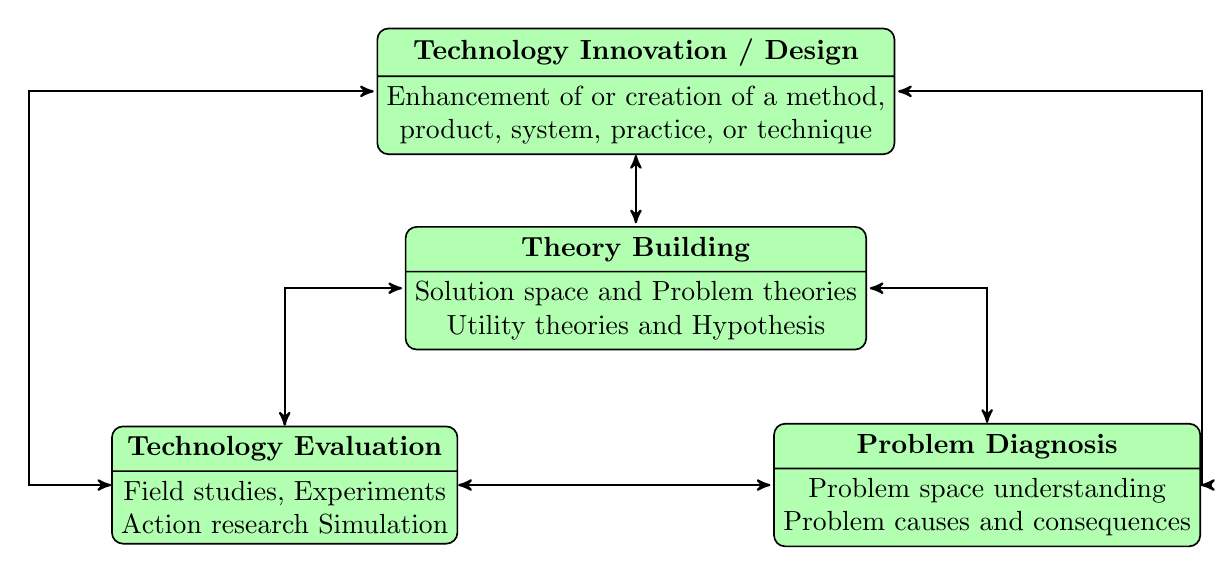
\begin{tikzpicture}[scale=0.50, ->, >=stealth', shorten >=1pt, node distance=6cm, semithick,
			every state/.style={rectangle, text centered, rounded corners, black, draw=black, fill=green!30, minimum width=2cm,minimum height=1.2cm,}]
			
			\node[state] (TechEval) [align=center, rectangle split, rectangle split parts=2] 
			{\textbf{Technology Evaluation} \nodepart{second} Field studies, Experiments \\ Action research Simulation};
			
			\node[state] (ProbDiag) [right=4cm of TechEval, align=center, rectangle split, rectangle split parts=2] 
			{\textbf{Problem Diagnosis} \nodepart{second} Problem space understanding \\ Problem causes and consequences};
			
			\node[state] (TechInnovDesg) [yshift=5cm, align=center, rectangle split, rectangle split parts=2] at ($(TechEval)!0.5!(ProbDiag)$)
			{\textbf{Technology Innovation / Design} \nodepart{second} Enhancement of or creation of a method, \\ product, system, practice, or technique};
			
			\node[state] (TheoryBld) [below of=TechInnovDesg, yshift=3.5cm, align=center, rectangle split, rectangle split parts=2]
			{\textbf{Theory Building} \nodepart{second} Solution space and Problem theories \\ Utility theories and Hypothesis};
			
			\draw[<->, thick] (TechInnovDesg.south) -- (TheoryBld.north);
			\draw[<->, thick] (TechEval.east) -- (ProbDiag.west);
			\draw[<->, thick] (TechEval.west) -| (-6.5,1.5) |- (TechInnovDesg.west);
			\draw[<->, thick] (TechEval.north) |- (TheoryBld.west);
			\draw[<->, thick] (ProbDiag.east) -| (23.3,1.5) |- (TechInnovDesg.east);
			\draw[<->, thick] (ProbDiag.north) |- (TheoryBld.east);
			
		\end{tikzpicture}
	\end{center}
	\caption{An activity framework for design science research \cite{Kuechler01102008}.}
	\label{fig:designscienceframework}
\end{figure}

%	\begin{figure}
	%		\begin{center}
		%			
\includegraphics[width=3.5in, height=2.5in]{images/Methodology_original}
		%			\caption{An Activity Framework for Design Science Research}
		%			\label{fig:designscienceframework}
		%		\end{center}
	%	\end{figure}

\section{Image Selection Methodology}\label{Image_Selection_Methodology}

%At the age of interactive information system, digital icons or pictorial signs plays an important role conveying information quickly in contrast to use of text. Universally accepted icons also can break written language, cultural barriers, and convey large amount of information efficiently and concisely \cite{COLLAUD2022102290} \cite{doi:10.1177/2041669518780807} \cite{doi:10.1177/2041669518780807}. Moreover, as mentioned in Section XXX, human can process visually presented information more quickly over text based approach. 

%While innovating our VFS, identified limitations in the existing contributions and through theory building component of the DRSR methodology, we proposed different user VFS users.

%While appropriate image can transfer information at a lighting speed increasing completeness and readability of documents, inappropriate one may result poor result especially in e-commerce where icon or image selection affects click-through rate \cite{Hyun2022} \cite{10.1145/3543873.3584646}. Although in this work, we are not going to design any icons for our proposed VFS; rather we will use most commonly used icons, We need to select icons carefully with the intention of avoiding misinterpretation. We aligned our icon selection strategy with icon design standard discussed by Collaud et al. \cite{COLLAUD2022102290}. These are access to meaning, familiarity, visual complexity, and aesthetic appeal  \cite{COLLAUD2022102290}.

	Using appropriate images can significantly enhance document clarity and readability by conveying information quickly. Conversely, poorly chosen visuals can lead to negative outcomes, particularly in e-commerce, where icon or image selection directly impacts click-through rates \cite{Hyun2022} \cite{10.1145/3543873.3584646}. In this work, we will not design custom icons for our proposed VFS; instead, we will rely on widely used icons. However, careful selection is essential to prevent misinterpretation. Our icon selection strategy follows the design standards outlined by Collaud et al. , focusing on four key principles: meaningfulness, familiarity, visual complexity, and aesthetic appeal \cite{COLLAUD2022102290}.
	


%[Icons play an important role in our daily lives. As
%pictorial signs, they express words, functions, or instructions in a nonverbal
%language. We see them at the train station, at the airport, in the
%museum, at the workplace, on the road as well as on almost every
%interactive user interface [e.g., [5–7]]. One reason for the extensive use
%of iconic representations is their ability to make actions, objects, or
%concepts easier to find, recognize, learn, and remember compared to the
%use of text [8–11]. In addition, icons are considered to be better understood
%by illiterate users or members of different language groups
%
%The literature highlights four key characteristics used by a variety of
%icon designs; access to meaning, familiarity, visual complexity, and aesthetic
%appeal
%
%] \cite{COLLAUD2022102290}
%
%
%[With the improvement of informationization as well as the development of human–computer
%interactions, icons have become an important component of digital user interfaces
%(Li, Chen, Sha, \& Lu, 2017; Nakamura \& Zeng-Treitler, 2012). Compared with words,
%graphic symbols are able to transcend language barriers
%
%In general, when designers create an icon, three icon characteristics need to be taken into
%consideration: visual complexity, concreteness, and semantic distance
%
%]\cite{doi:10.1177/2041669518780807}
%
%[In e-commerce, images are widely used to display more intuitive information about items, and image selection greatly afects the click-through rate (CTR) of users.
%
%
%]\cite{10.1145/3543873.3584646}

%[Compared with words, graphic symbols are able to transcend language barriers and convey large amounts of information in a more concise and efficient way
%
%However, people are still likely to misinterpret the meanings of icons that are poorly
%designed.
%
%To date, numerous studies investigated the effects of these icon characteristics on
%visual search performance: people responded more quickly and more accurately to simple
%icons than complex icons , users were more efficient at
%understanding concrete icons compared with abstract icons
%
%However, a few researchers noticed that performance differences between different icon types
%diminished after users had gained considerable experience with the icons . McDougall et al. (2000) conducted a series of experiments to examine the
%factors considered central to icon usability. The findings indicated that performance
%differences between concrete and abstract icons diminished after icon sets were used more
%frequently. To further explore this issue, Isherwood, McDougall, and Curry (2007)
%experimented with an icon identification task over a long series of trials to mimic the
%effects of increasing user experience.
%
%]\cite{doi:10.1177/2041669518780807}

%[Image selection system also plays an important role
%in automatic report generation as insertion of appropriate images can increase the
%completeness and readability of the report.] \cite{Hyun2022}	
	
	
\section{User Group Identification}	

%	Although there is no doubt that an FS is an important methodology for achieving the true goal for responsible AI (iff properly executed), the term FS itself is somewhat elusive, overused, and sometimes misunderstood. There must be a clear, comprehensive and actionable definition of FS for RAI. An FS for an AI service can be a long, text heavy document capturing all relevant attributes categorized in one or multiple sections \cite{arnold_factsheets_2018}. We believe a comprehensive single FS is not sufficient for all audiences. For an ML service or an application, we believe there are four user groups and proposing four types of FS, one for each:

%To identify distinct FS user group, we were inspired by the contribution made by Arnold et al., Michell et al., Gebru et al., and Kasia et al.. They all included ML developers e.g., data scientist (DS), quality assurance (QA) personnel, a potential FS user. It is our understanding that Kasia et al. considered these user group as AI practitioners, Arnold et al. considered \enquote{users} as technical user not end users and Kasia et al. considered policy makers as person holding a public office. Except the mentioned user groups, Arnold et al. considered Auditors and Kasia et al. policymakers as a potential FS user group. We identified and categorized our proposed user in four groups. We believe business executives should be in the same group as policymakers as they make decisions for their respective company. We accepted Auditor group as is but included all technical groups e.g. DS, ML developer, QA personnel, AI practitioners etc., under one unified group, i.e., \enquote{Developers}. At the end, we introduce a new group which was not previously considered, i.e., end user.

%To distinguish the various FS user groups, we were inspired by the work of Arnold et al., Michell et al., Gebru et al., and Kasia et al. These studies commonly included ML professionals, e.g., data scientists (DS) and quality assurance (QA) personnel as potential FS users. Based on our interpretation, Kasia et al. classified these individuals as AI practitioners while Arnold et al. viewed them as technical users rather than end users. Additionally, Kasia et al. defined policymakers as individuals holding public office. Beyond these groups, Arnold et al. identified auditors, and Kasia et al. included policymakers as potential FS users.
%
%In our approach, we organized the proposed users into four categories. We grouped business executives with policymakers, as both make strategic decision. We retained the auditor category as is but consolidated all technical roles mentioned above into a single group labeled “Developers.” Finally, we introduced a new category not previously considered, i.e., end users.

	To differentiate the various FS user groups, we drew inspiration from the work of Arnold et al., Michell et al., Gebru et al., and Kasia et al. These studies often identified machine learning (ML) professionals—such as data scientists (DS) and quality assurance (QA) specialists—as potential FS users. Kasia et al. classified these individuals as AI practitioners, whereas Arnold et al. considered them technical users rather than end users. Kasia et al. also defined policymakers as those holding public office. Beyond these groups, Arnold et al. included auditors, while Kasia et al. listed policymakers as potential FS users.

	In our framework, we organized the proposed users into four categories. Business executives were grouped with policymakers, as both play strategic decision-making roles. We retained auditors as a distinct category but combined all technical roles into a single group labeled “Developers.” Finally, we introduced a new category not previously considered: end users.



%	\begin{multicols}{2}
%		\begin{enumerate}[label={\arabic*.}]
	\begin{itemize}
		\item Policymaker / Business Executive;
		\item Auditor;
		\item Developer; and
		\item End user.
	\end{itemize}
%		\end{enumerate}
%	\end{multicols}

\subsection{Policymaker / Business Executive:}

%	Policymakers are responsible for making decisions on complex issues. In many cases, especially in science and technology, they often have limited or no understanding of a problem and proposed solution yet they have to make a decision about its potential usage. Policymakers focus more on the impact of a certain technology to the general population, effectiveness of the solution solving a problem and whether there is a possible violation of law. For in depth technical analysis, policy makers are becoming more reliant on their advisors \cite{thomas_expertise_2013}. Keeping their priorities in mind, we propose the below FS definition intended for policymakers.
	
	Policymakers face the challenge of making decisions on complex issues, particularly in areas like science and technology, where they often have limited understanding of the problems and proposed solutions. Despite this, they must determine whether and how a technology should be used. Their focus typically lies on its potential impact on the public, its effectiveness in addressing the issue, and any possible legal implications. For detailed technical evaluations, policymakers increasingly depend on expert advisors \cite{thomas_expertise_2013}. With these priorities in mind, we propose the following FS definition tailored for policymakers.
	
%	\textbf{Definition 1: }\textit{An FS is a single or multi-page document, preferably less text heavy, that provides a high-level overview of an ML model. The document should provide legal constraints, known security limitations, applicable domains, data sources, one or more basic usage examples, and how AI trustworthiness was achieved. The document should also contain possible risk analysis in cases of misuse.}
	
	\textbf{Definition 1: }\textit{A Fact Sheet (FS) is a concise, single- or multi-page document that offers a high-level summary of a machine learning (ML) model. It should outline legal requirements, known security limitations, relevant application domains, data sources, and include one or more basic usage examples. Additionally, the FS must explain how AI trustworthiness was established and provide a risk assessment for potential misuse.}
	

\subsection{Auditor:}

%	Audit is an integral part of RAI; mandatory to ensure fairness, accountability, transparency, and trustworthiness for any AIS. We believe an FS generated for auditors can play a pivotal role to achieve governance. While policymakers focus on high-level contents of an FS, auditors focus on each high-level item along with other technical details. Auditors ensure from the theoretical aspect that the AIS is able to solve one or more problems that it claims it can solve by maintaining RAI and GDPR policies, and does not violate any other applicable regulations. It is the auditors job to ensure the AIS provides all necessary documentation and other materials to support their claims. We are proposing the below FS definition intended for auditors.
	
%	Auditing is a critical component of RAI, essential for ensuring fairness, accountability, transparency, and trustworthiness in any AIS. A well-structured FS designed for auditors can play a key role in achieving these governance objectives. While policymakers typically concentrate on the high-level elements of an FS, auditors delve deeper into each item and its technical details. Their responsibility is to verify, from a theoretical standpoint, that the AIS can effectively address the problems it claims to solve, while adhering to RAI and GDPR policies and avoiding violations of other applicable regulations. Auditors must also confirm that the AIS provides all necessary documentation and supporting materials for its claims. To facilitate this process, we propose the following FS definition specifically intended for auditors.
	Auditing is a vital aspect of Responsible AI (RAI), ensuring fairness, accountability, transparency, and trust in any Artificial Intelligence System (AIS). A well-structured Fact Sheet (FS) tailored for auditors plays a crucial role in meeting these governance objectives. While policymakers often focus on high-level FS components, auditors examine each element in detail, including its technical aspects. Their task is to confirm, from a theoretical perspective, that the AIS can effectively solve the problems it claims to address, complies with RAI and GDPR requirements, and avoids breaches of other relevant regulations. Auditors must also verify that the AIS provides complete documentation and supporting evidence for its claims. To support this process, we propose the following FS definition specifically designed for auditors.

	
%	\textbf{Definition 2: }\textit{An FS is a multi-page document often generated periodically during machine learning development or update life-cycle. The document should contain in-depth technical, legal, possibly all use-cases with one or more examples, data usage, known security limitations, applicable domains, and explanations about how AI trustworthiness was achieved for an AIS. The document should also contain the source of each technology used, technological gap (if any), and sample data (both in original and processed form) with explanation(s) of how fairness and unbiasness was achieved.}

	\textbf{Definition 2: }\textit{A Fact Sheet (FS) is a detailed, multi-page document typically prepared at regular intervals during the development or update cycle of a machine learning system. It should include comprehensive technical and legal information, all relevant use cases with examples, data usage details, known security limitations, applicable domains, and an explanation of how trustworthiness was established for the AI system. Additionally, the FS should specify the source of each technology used, identify any technological gaps, and provide sample data—both in its original and processed forms—along with explanations of how fairness and impartiality were ensured.}



\subsection{Developer:}

%	AISs are highly-complex data-driven technological innovations or inventions. Collecting data is the very first step for developing an AIS and developers need to do much work to make the collected data usable for training an ML model. Developers must ensure that collected data is unbiased, fair, complete, consistent, and free from personal identifiable information (PII). In summary the data maintains all legal regulations, e.g., General Data Protection Regulations (GDPR). The development team must ensure that all decisions or recommendations coming from the model are explainable and most importantly free from bias. As mentioned there can still be biased data in the dataset so the development team must take extra caution and put extra measures in place to catch those. It is also possible that the model development algorithm can have biased logic; intentionally or unintentionally. While the development team should always keep an eye on the overall model’s performance, they also must audit and monitor what logic is going into model development. They must also ensure that they know who and how those changes (if any) were made. 

%	AI Models are living software as they are data driven. This unique property makes them vulnerable over time. This means an AI Model requires continuous monitoring. Models can lose or gradually decrease their performance; drift management and performance monitoring are a must for all serving AI Models. It is also a mandatory requirement to retrain and remodel a Model if required.  Enlightened by the above discussion, we are proposing the below FS definition intended for ML developers.
	
%	AIS are complex, data-driven technologies. The first step in developing an AIS is data collection, followed by extensive work to prepare that data for training ML models. Developers must ensure the data is unbiased, fair, complete, consistent, and free from personally identifiable information (PII), while complying with legal standards such as the GDPR. It is critical that all outputs—whether decisions or recommendations—are explainable and free from bias. Since datasets may still contain hidden biases, development teams must implement additional safeguards to detect and mitigate them. Furthermore, algorithms themselves can introduce bias, whether intentional or accidental. Teams should continuously monitor model performance and audit the logic behind its development, maintaining clear records of any changes and who made them.
%	
%	AI models are dynamic and evolve over time because they are data-driven. This makes them vulnerable to performance degradation, requiring ongoing monitoring and drift management. Retraining and updating models when necessary is essential to maintain reliability and effectiveness. Based on these considerations, we propose the following FS definition for ML developers.

	Artificial Intelligence Systems (AIS) are sophisticated, data-driven technologies. Their development begins with data collection, followed by extensive preparation to make the data suitable for training machine learning (ML) models. Developers must ensure that the data is fair, unbiased, complete, consistent, and free of personally identifiable information (PII), while adhering to legal requirements such as GDPR. All outputs—whether decisions or recommendations—must be explainable and unbiased. Because hidden biases can still exist in datasets, development teams should implement safeguards to detect and mitigate them. Additionally, algorithms themselves may introduce bias, whether intentional or accidental. Continuous monitoring of model performance and auditing the development logic are essential, along with maintaining detailed records of all changes and their authors.
	
	AI models are dynamic and evolve over time due to their reliance on data, making them susceptible to performance degradation. This requires ongoing monitoring and management of model drift. Regular retraining and updates are critical to ensure reliability and effectiveness. Based on these factors, we propose the following FS definition for ML developers.
	
	
	
	\textbf{Definition 3: }\textit{An FS is a comprehensive, multi-page technical document typically prepared periodically or on an ad-hoc basis during the development, modification, or life-cycle updates of machine learning models. It should detail every step involved in creating the ML model, including how training data was sourced, processed, and the technologies used to prepare it for use. The document must list all algorithms applied, provide in-depth technical justifications for their selection, and outline potential drawbacks, limitations, and any security concerns. Additionally, it should include evidence of the model’s effectiveness, performance metrics, and the approach taken for future updates or upgrades.}

%	\textbf{Definition 3: }\textit{An FS is a multi-page, in-depth, highly-technical document often generated periodically or on an ad-hoc basis during machine learning development, modification, or life-cycle update. This document should contain each and every step taken for developing an ML model. This includes how training data was acquired, processed, and technologies used for making it ready for further use. The document should contain all ML algorithms used for developing a model, detailed technical explanations of why they are suitable, possible drawbacks, limitations, and security concerns (if any). It also should provide sufficient evidence on the efficiency of a model, performance metrics, and strategy used for updating or upgrading a model.}

\subsection{End user:}

%	End-users of an AIS are generally less tech-savvy. They are less concerned about the inner complexities of the services they use for making their life easier. We believe an AIS provider must inform all end users in their own language, or in plain English, about their contribution for enhancing or updating the AIS services. Traditionally end-users can decide whether they want a report from an application about its usage or crash log, but in general an AIS automatically generates those data. We believe the majority of end users have little or no knowledge about this activity. Keeping end-user technical ability and requirements in mind, we are proposing the below FS definition intended for ML users.
	
	End-users of an AIS are typically less technically inclined and generally unconcerned with the underlying complexities of the systems they use to simplify their lives. We believe AIS providers should clearly communicate, in plain language or simple English, how users contribute to improving or updating AIS services. Traditionally, users could choose whether to share reports on application usage or crash logs, but AIS often collects such data automatically. Most users are likely unaware of this process. Considering the technical limitations and needs of end-users, we propose the following FS definition specifically designed for ML users.

	\textbf{Definition 4: }\textit{An FS is a single or multi-page, reasonably short and less technical document generated periodically (as necessary) for AIS users. The document should contain all use-cases with one or more examples, rights and responsibilities of the users for using an AIS, and possible security concerns and limitations.}

\section{Visual FactSheet}

	Data is the fuel for any ML model. Training data acted as a input for ML model and dictates how it will perform while providing recommendation. There is a common notion that the more data that a ML is trained on, the more it will perform accurately \cite{nield2022essential}. Hence, data became the new currency in today's interconnected world\cite{Gates:2014:DNC:2683467.2683477}. Due to this reason, we concluded user should know what data they are sharing, how the provided will retain, process, and share their data.
	
	While designing our VFS template, we took a risk based approach. For ML development, there are mainly two type of risks, i.e., data level and model level risk. Data risk encapsulates data bias, shift, adversarial attack, etc. while model level risk includes accuracy, uncertainty, etc. \cite{ZHANG2022113800}. Instead of treating them separately we took an hybrid approach combining model and data bias and fairness risk into two, accuracy solely for model, and leave a wide range for any other risk the provider may consider informing to it users.

	\enquote{A Picture Is Worth a Thousand Words} \cite{sullivan_picture_2017}. Visual depiction of complex agreements not only provides clarity of the content but also can enhance a nontechnical person's decision making process \cite{suters_emergence_2023} \cite{kim_impact_2021}. While the use of visual depictions over text-heavy content makes it easier to understand product instructions for many companies, it is uncommon to use the same strategy for capturing a user's response of proper understating to the license agreement despite their possible effectiveness for improving information quality, credibility, and enhance the decision making process \cite{kim_impact_2021}. We expect a VFS will be a useful approach to inform license information pictorially. We propose the most important items in a VFS for end-users:
%	\begin{multicols}{2}
%		\begin{enumerate}[label={\arabic*.}]
	\begin{itemize}
		\item Purpose;
		\item Data Collection;
		\item Data Processing;
		\item Data Retention;
		\item Data Share;
		\item Accuracy, Fairness, Bias; and 
		\item Potential Risk.
	\end{itemize}
%		\end{enumerate}
%	\end{multicols}

	A VFS should begin by clearly stating the purpose of the AIS service, including an example problem and how the service addresses it. Users must be informed about the types of data the AIS provider may collect during usage. While providing examples of collected data is optional, it is strongly recommended. At the very least, the provider should confirm whether data collection occurs with a clear \enquote{Yes} or \enquote{No}. If data collection is confirmed, the provider must explain why the data is collected and how it will be used in the future. Additionally, the provider should specify measures taken to ensure that no personally identifiable information (PII) is included, again with a simple \enquote{Yes} or \enquote{No} acknowledgment.
	
	If user data is collected and processed, the provider must disclose its data retention policy and explain how data will be securely destroyed after the retention period ends. AIS providers often share collected data with affiliates, government agencies (such as law enforcement), and other third-party AIS providers. In cases of business transfers, ownership of this data may also change. Providers must clearly identify who will receive the data and whether it will be shared in raw or processed form.	Regardless of whether the service is free or paid, AIS providers should present evidence of the effectiveness and value of their offerings. For AIS, the accuracy of underlying machine learning models is a key metric. Given concerns about bias and fairness, providers must inform users about the level of impartiality in their service, including reported percentiles for accuracy, fairness, and bias.

	Finally, AIS services are not without risks. There is growing concern about adversarial attacks on ML models, as well as threats like data poisoning, model theft, and hijacking. Providers must acknowledge these potential risks and explain the steps taken to minimize or eliminate them.



%\subsection{Purpose:}

%	A VFS must start with the purpose of the AIS service. This should provide an example problem and how the AIS service is solving it.
%
%%\subsection{Data Collection:}
%
%%	An AIS user must know what type of data the AIS provider will be collecting (if any) while using it. The AIS provider may or may not provide an example informing the user what type of data will be collected. It is highly recommended that the AIS provider will provide an example. The minimum requirement of this step can be an acknowledgment from the AIS provider in the form of a \enquote{Yes} or \enquote{No}.
%	
%	AIS users should be informed about the types of data an AIS provider may collect during usage. While the provider might choose to include examples of the data collected, doing so is strongly recommended. At a minimum, the provider should acknowledge whether data collection occurs by providing a clear \enquote{Yes} or \enquote{No} response.
%	
%
%%\subsection{Data Processing:}
%
%%	If the AIS provider acknowledges that they collect user data, the provider must inform users why they collect it and how user data will be processed for future use. The provider must also inform users how they make sure collected data is free from PII. The minimum requirement of this step can be an acknowledgment from the AIS provider as a form of a \enquote{Yes} or \enquote{No}.
%	
%	If an AIS provider confirms that it collects user data, it must explain the purpose of the collection and how the data will be used in the future. Additionally, the provider should clarify the measures taken to ensure that the collected data does not contain any personally identifiable information (PII). At a minimum, this step requires the provider to give a simple \enquote{Yes} or \enquote{No} acknowledgment.
%
%%\subsection{Data Retention:}
%
%%	If the AIS provider collects and processes user data, the provider must inform users of their data retention policy. They must also inform users how they destroy user data once the retention period is over.
%	
%	If an AIS provider collects and processes user data, it must clearly inform users about its data retention policy. Additionally, the provider should explain how user data will be securely destroyed once the retention period ends.
%
%%\subsection{Data Share:}
%
%%	AIS providers often share collected data with their affiliates, government organizations, e.g., law enforcement agencies, and third party AIS providers. They also share and transfer ownership of collected data in the occurrence of business transfer. It is necessary for the provider to inform users with whom they intend to share collected data and in what form, i.e., unprocessed or processed. 
%	
%	AIS providers frequently share collected data with affiliates, government bodies such as law enforcement agencies, and other third-party AIS providers. In cases of business transfers, ownership of this data may also be transferred. Providers must clearly inform users about who will receive the data and specify whether it will be shared in its raw or processed form.
%	
%
%%\subsection{Accuracy, Fairness, and Bias:}
%
%%	Regardless of free or paid services, it is mandatory for the AIS provider to show evidence about the effectiveness and usefulness of the service they are offering. For AIS underlying ML models' accuracy is a widely accepted metric for such \cite{blagec_critical_2020}. Since there is a concern about unfair and biased recommendations or decisions, it is the provider's responsibility to inform its users of the level of fair and unbiased recommendations or decisions of their service. The minimum requirement of this step can be a percentile of accuracy, fairness, and biasness. 
%	
%	Whether the service is free or paid, AIS providers must present evidence demonstrating the effectiveness and value of their offerings. For AIS, the accuracy of underlying ML models is widely recognized as a key metric \cite{blagec_critical_2020}. Given concerns about biased or unfair recommendations and decisions, providers are responsible for informing users about the degree of fairness and impartiality in their service. At a minimum, this should include a reported percentile for accuracy, fairness, and bias.
%
%%\subsection{Potential Risk:}
%
%	AISs are not free from potential risk. There is a growing concern about adversarial attacks on the underlying ML models along with training data poisoning, stealing, and model hijacking. The AIS provider must acknowledge if there is any potential risk for using the service and how the provider minimizes or eliminates those potential risks.

\section{VFS Example}

	We present two examples of a VFS: We chose to use ChatGPT and Grammarly. These are two of the most popular free AISs. We want to apply our VFS concept and justify the usefulness of our proposed approach for AIS users.

\subsection{ChatGPT}

	ChatGPT is a LLM-based chatbot capable of processing natural language and offers a human-like conversation service designed to assist with tasks and answer questions \cite{ortiz_what_nodate}. Introduced by OpenAI and available to the public since November 2022, the service gained popularity very quickly and has affected almost every field. We evaluated the \enquote{Privacy Policy} and prepared the VFS shown in Figure \ref{fig:ChatGPT}. Appendix \ref{appendix:a} provide legends for icons used in Figure \ref{fig:ChatGPT} and Figure \ref{fig:Grammarly}.

	In the \enquote{Collect} section of Figure \ref{fig:ChatGPT}, we present pictorially the type of data OpenAI is collecting while users engage with their service. We identified that ChatGPT automatically collects all information. This includes personal and social media information, device information from where the service is used, and all types of communication messages. They also run real time analytics on the collected data and claim to provide a better experience while using the ChatGPT service \cite{openai_privacy_2023}. In a similar fashion, the sections \enquote{Process}, \enquote{Share}, and \enquote{Retention Period} of Figure \ref{fig:ChatGPT} visually shows that OpenAI retains user data for an infinite time. OpenAI processes those data for their research, developing new products or services, and improving existing services. The company also says they may or do share user data with government agencies, third party vendors, and their affiliated companies \cite{openai_privacy_2023}. Although the core of ChatGPT is an ML model using LLM technology, there is no publicly available information about the model. We did not find any evidence about its accuracy, potential risk of using the ChatGPT service, and data fairness and biasness of the data that the underlying ML model is trained on.
	
	
	\begin{table}
			\centering
			\begin{tabular}{|l|l|c|}
					\hline
					\multicolumn{3}{|l|}{\specialcell{ChatGPT is one of the most popular AIS. It is a LLM-based chatbot capable of processing natural \\language and offers human-like conversation service design to assist with tasks and answer questions.}} \\
					\hline
%					\multicolumn{3}{|c|}{\textbf{Data}} \\
%					\hline
					Activity & Status & Activity Details\\
					\hline
					Collect & 
\includegraphics[width=8mm,scale=0.5]{images/check} & \specialcell{
						
\includegraphics[width=8mm,scale=0.5]{images/socialmedia} 
						
\includegraphics[width=8mm,scale=0.5]{images/personalinformation} 
						
\includegraphics[width=8mm,scale=0.5]{images/usergeneratedcontent} 
						
\includegraphics[width=8mm,scale=0.5]{images/usercommunication} 
						
\includegraphics[width=8mm,scale=0.5]{images/logfile}  
						
\includegraphics[width=8mm,scale=0.5]{images/datausage} 
						
\includegraphics[width=8mm,scale=0.5]{images/deviceinformation} 
						
\includegraphics[width=8mm,scale=0.5]{images/httpcookie}
						
\includegraphics[width=8mm,scale=0.5]{images/analytics} 
						
\includegraphics[width=8mm,scale=0.5]{images/additionalinformation} } \\
					\hline
					Process & 
\includegraphics[width=8mm,scale=0.5]{images/check} & \specialcell{
						
\includegraphics[width=8mm,scale=0.5]{images/research} 
						
\includegraphics[width=8mm,scale=0.5]{images/improvement} 
						
\includegraphics[width=8mm,scale=0.5]{images/newproduct} } \\
					\hline
					Share & 
\includegraphics[width=8mm,scale=0.5]{images/check} & \specialcell{
						
\includegraphics[width=8mm,scale=0.5]{images/thirdparty} 
						
\includegraphics[width=8mm,scale=0.5]{images/lawenforcement} 
						
\includegraphics[width=8mm,scale=0.5]{images/affiliate} } \\
					\hline
					\specialcell{Retention \\ Period} & 
\includegraphics[width=6.5mm,scale=0.4]{images/maybe} & \specialcell{
						
\includegraphics[width=8mm,scale=0.5]{images/retention} 
						
\includegraphics[width=8mm,scale=0.5]{images/unknown} } \\
					\hline
					\multicolumn{3}{|c|}{\textbf{Performance and Governance}} \\
					\hline
					Accuracy & 
\includegraphics[width=8mm,scale=0.5]{images/no} & \specialcell{
						
\includegraphics[width=8mm,scale=0.5]{images/unknown} } \\
					\hline
					Fairness & 
\includegraphics[width=8mm,scale=0.5]{images/no} & \specialcell{
						
\includegraphics[width=8mm,scale=0.5]{images/unknown} } \\
					\hline
					Bias & 
\includegraphics[width=8mm,scale=0.5]{images/no} & \specialcell{
						
\includegraphics[width=8mm,scale=0.5]{images/unknown} } \\
					\hline
					\specialcell{Potential \\ Risk} & 
\includegraphics[width=6.5mm,scale=0.4]{images/maybe} & \specialcell{
						
\includegraphics[width=8mm,scale=0.5]{images/unknown} } \\
					\hline
				\end{tabular}
			\caption{Visual FactSheet for ChatGPT }
%			\Description{Visual FactSheet for ChatGPT}
			\label{fig:ChatGPT}
		\end{table}
	
	
%	\begin{figure}[]
%		\centering
%		\begin{tabular}{ |P{1.5cm}|P{1cm}|P{5cm}|  }
%			\hline
%			\multicolumn{3}{|P{7.5cm}|}{ChatGPT is one of the most popular AIS. It is a LLM-based chatbot capable of processing natural language and offers human-like conversation service design to assist with tasks and answer questions.} \\
%			\hline
%			\multicolumn{3}{|c|}{\textbf{Data}} \\
%			\hline
%			Activity & Status & Activity Details\\
%			\hline
%			Collect & 
\includegraphics[width=8mm,scale=0.5]{images/check} & \specialcell{
\includegraphics[width=8mm,scale=0.5]{images/socialmedia} 
\includegraphics[width=8mm,scale=0.5]{images/personalinformation} 
\includegraphics[width=8mm,scale=0.5]{images/usergeneratedcontent} 
\includegraphics[width=8mm,scale=0.5]{images/usercommunication} 
\includegraphics[width=8mm,scale=0.5]{images/logfile}\\ 
\includegraphics[width=8mm,scale=0.5]{images/datausage} 
\includegraphics[width=8mm,scale=0.5]{images/deviceinformation} 
\includegraphics[width=8mm,scale=0.5]{images/httpcookie}
%				
\includegraphics[width=8mm,scale=0.5]{images/analytics} 
\includegraphics[width=8mm,scale=0.5]{images/additionalinformation} } \\
%			\hline
%			Process & 
\includegraphics[width=8mm,scale=0.5]{images/check} & \specialcell{
\includegraphics[width=8mm,scale=0.5]{images/research} 
\includegraphics[width=8mm,scale=0.5]{images/improvement} 
\includegraphics[width=8mm,scale=0.5]{images/newproduct} } \\
%			\hline
%			Share & 
\includegraphics[width=8mm,scale=0.5]{images/check} & \specialcell{
\includegraphics[width=8mm,scale=0.5]{images/thirdparty} 
\includegraphics[width=8mm,scale=0.5]{images/lawenforcement} 
\includegraphics[width=8mm,scale=0.5]{images/affiliate} } \\
%			\hline
%			\specialcell{Retention \\ Period} & 
\includegraphics[width=6.5mm,scale=0.4]{images/maybe} & \specialcell{
\includegraphics[width=8mm,scale=0.5]{images/retention} 
\includegraphics[width=8mm,scale=0.5]{images/unknown} } \\
%			\hline
%			\multicolumn{3}{|c|}{\textbf{Performance and Governance}} \\
%			\hline
%			Accuracy & 
\includegraphics[width=8mm,scale=0.5]{images/no} & \specialcell{
\includegraphics[width=8mm,scale=0.5]{images/unknown} } \\
%			\hline
%			Fairness & 
\includegraphics[width=8mm,scale=0.5]{images/no} & \specialcell{
\includegraphics[width=8mm,scale=0.5]{images/unknown} } \\
%			\hline
%			Bias & 
\includegraphics[width=8mm,scale=0.5]{images/no} & \specialcell{
\includegraphics[width=8mm,scale=0.5]{images/unknown} } \\
%			\hline
%			\specialcell{Potential \\ Risk} & 
\includegraphics[width=6.5mm,scale=0.4]{images/maybe} & \specialcell{
\includegraphics[width=8mm,scale=0.5]{images/unknown} } \\
%			\hline
%		\end{tabular}
%		\caption{Visual FactSheet for ChatGPT }
%		\Description{Visual FactSheet for ChatGPT}
%		\label{fig:ChatGPT}
%	\end{figure}
%	
%	\begin{figure}[]
%		\centering
%		\begin{tabular}{ |P{1.5cm}|P{1cm}|P{5cm}|  }
%			\hline
%			\multicolumn{3}{|P{7.5cm}|}{Grammarly is an AI powered writing assistant that helps people communicate with confidence. It assists in improving the correctness, clarity, engagement, and delivery of a written document.} \\
%			\hline
%			\multicolumn{3}{|c|}{\textbf{Data}} \\
%			\hline
%			Activity & Status & Activity Details\\
%			\hline
%			Collect & 
\includegraphics[width=8mm,scale=0.5]{images/check} & \specialcell{
\includegraphics[width=8mm,scale=0.5]{images/socialmedia} 
\includegraphics[width=8mm,scale=0.5]{images/personalinformation} 			
\includegraphics[width=8mm,scale=0.5]{images/usergeneratedcontent} 
\includegraphics[width=8mm,scale=0.5]{images/usercommunication} 
\includegraphics[width=8mm,scale=0.5]{images/logfile}\\ 
\includegraphics[width=8mm,scale=0.5]{images/datausage} 
\includegraphics[width=8mm,scale=0.5]{images/deviceinformation} 
\includegraphics[width=8mm,scale=0.5]{images/httpcookie}
%				
\includegraphics[width=8mm,scale=0.5]{images/analytics} 
\includegraphics[width=8mm,scale=0.5]{images/additionalinformation} 
\includegraphics[width=8mm,scale=0.5]{images/payment} } \\
%			\hline
%			Process & 
\includegraphics[width=8mm,scale=0.5]{images/check} & \specialcell{
\includegraphics[width=8mm,scale=0.5]{images/research} 
\includegraphics[width=8mm,scale=0.5]{images/improvement} 
\includegraphics[width=8mm,scale=0.5]{images/newproduct} } \\
%			\hline
%			Share & 
\includegraphics[width=8mm,scale=0.5]{images/check} & \specialcell{
\includegraphics[width=8mm,scale=0.5]{images/thirdparty} 
\includegraphics[width=8mm,scale=0.5]{images/lawenforcement} 
\includegraphics[width=8mm,scale=0.5]{images/affiliate} 
\includegraphics[width=8mm,scale=0.5]{images/bank} } \\
%			\hline
%			\specialcell{Retention \\ Period} & 
\includegraphics[width=6.5mm,scale=0.4]{images/maybe} & \specialcell{
\includegraphics[width=8mm,scale=0.5]{images/retention} 
\includegraphics[width=8mm,scale=0.5]{images/unknown} } \\
%			\hline
%			\multicolumn{3}{|c|}{\textbf{Performance and Governance}} \\
%			\hline
%			Accuracy & 
\includegraphics[width=8mm,scale=0.5]{images/no} & \specialcell{
\includegraphics[width=8mm,scale=0.5]{images/unknown} } \\
%			\hline
%			Fairness & 
\includegraphics[width=8mm,scale=0.5]{images/no} & \specialcell{
\includegraphics[width=8mm,scale=0.5]{images/unknown} } \\
%			\hline
%			Bias & 
\includegraphics[width=8mm,scale=0.5]{images/no} & \specialcell{
\includegraphics[width=8mm,scale=0.5]{images/unknown} } \\
%			\hline
%			\specialcell{Potential \\ Risk} & 
\includegraphics[width=6.5mm,scale=0.4]{images/maybe} & \specialcell{
\includegraphics[width=8mm,scale=0.5]{images/unknown} } \\
%			\hline
%		\end{tabular}
%		\caption{Visual FactSheet for Grammarly }
%		\Description{Visual FactSheet for Grammarly}
%		\label{fig:Grammarly}
%	\end{figure}

%	\begin{figure*}[t!]
%		\centering
%		\begin{subfigure}[t]{0.5\textwidth}
%			\centering
%			
\includegraphics[height=3in]{images/ChatGPT}
%			\caption{Visual FactSheet for ChatGPT }
%			\label{fig:ChatGPT}
%		\end{subfigure}%
%		
%		\begin{subfigure}[t]{0.5\textwidth}
%			\centering
%			
\includegraphics[height=3in]{images/Grammarly}
%			\caption{Visual FactSheet for Grammarly }
%			\label{fig:Grammarly}
%		\end{subfigure}
%		\caption{Visual FactSheet}
%	\end{figure*}

%\subsection{Grammarly}

%	Grammarly is an AI-powered writing assistant. It is an advanced technology that claims to improve correctness and clarity of a written document or assist while writing \cite{grammarly_what_nodate}. Launched in 2009 as a free or paid service, it is becoming a popular writing assistant among students and the general population.  We evaluated the \enquote{Terms of Service}, and \enquote{Privacy Policy} and prepared the VFS shown in Figure \ref{fig:Grammarly}. The VFS for Grammarly is very similar to that of ChatGPT except Grammarly also collects and processes payment information. This payment information collection applies only for their paid users \cite{grammarly_privacy_2023}.
	
\section{Survey Design}

We designed our survey using guidelines mentioned by Arlene Fink \cite{alma991013701999705153}

\subsection{Survey Questions}

Surveys are data collection methods use to obtain information from and about people: From and about which people, how often and when.

Survey method: Online questionnaire

regardless of your survey's design or size, you must think ahead to how you plan to analyze the survey's data 

the overwhelming majory of surveys rely on multiple-choice questions because they have proven themselves to be the more efficient and ultimately more reliable. Their efficiency comes from being easy to use, score, and enter data. Also, their reliability is enhanced because of the uniform data they provided; everyone responds in terms of the same options

\begin{itemize}
	\item What is your level of education?
	\item Your current or previous education background?
	\item Are you a Computer Science Student?
	\item How familiar are you with AI?
	\item Do you use social media platform (s)?
	\item Do you or have you ever use ChatGPT or Grammerly or Microsoft Co-Pilot or any other writing assistance tool?
	
	Now, show them the license agreement?
	
	\item do you know what information will the application will share?
	\item After reading the agreement, how comfortable are you using the application
	
	Now, show them the VFS, and ask the same question.
	
\end{itemize}



%	The study adopted a cross-sectional design. To analyze the information landscape encountered by a typical patient, this study simulated a common online information-seeking process. Given that the methodology relied entirely on the analysis of publicly available data, it did not involve human participants or animal subjects. This study focuses solely on the content and presentation of information, not on direct patient-level outcomes such as comprehension, behavioral change, or adherence, which are acknowledged as limitations. Consequently, approval from an Institutional Review Board was exempt.

\subsection{Survey Result}

TBD

\section{Conclusion and Limitation}

	In this paper, we proposed four FS definitions by identifying and categorizing four user groups and introduced a methodology for creating a VFS for ML services. We believe our proposed FS definitions will be able to reduce confusion for FS generators or creators. We also believe that the proposed VFS will benefit a growing number of ML service consumers protecting their rights and making informed decisions when using publicly available free ML services. We hope to continue our work on VFS and use it as an integral part of an ML service or project and show the effectiveness of the proposed methodology. Although we introduced four types of VFS with definitions, we concentrated our focus on the end-user type. All icons used in this paper for preparing VFS are publicly available, in generic form, and downloaded from Flaticon.com. We believe there is an opportunity for standardizing icons used in this paper. We also hope to conduct a survey experiment to identify the strength and weakness of our proposed VFS and continue our contribution on icons standardization effort.
	
%	In this paper, we present four definitions of FS by identifying and classifying four distinct user groups, along with a methodology for developing a VFS tailored for ML services. Our proposed FS definitions aim to minimize confusion among FS creators and generators. Furthermore, we believe the VFS framework will empower an increasing number of ML service consumers by safeguarding their rights and enabling informed decisions when using publicly available free ML services. Moving forward, we plan to integrate VFS into ML services or projects and demonstrate the effectiveness of our approach. Although we introduced four VFS types with corresponding definitions, our primary focus was on the end-user category. All icons utilized in this paper to design VFS are generic, publicly accessible, and sourced from Flaticon.com. We see potential for standardizing these icons and intend to conduct a survey to evaluate the strengths and weaknesses of our proposed VFS, continuing our efforts toward icon standardization.

\section{Acknowledgments}

%%
%% The next two lines define the bibliography style to be used, and
%% the bibliography file.
\bibliographystyle{ACM-Reference-Format}
\bibliography{facct}


%%
%% If your work has an appendix, this is the place to put it.
\appendix

\section{Grammarly} \label{appendix:b}

Grammarly is an AI-powered writing assistant. It is an advanced technology that claims to improve correctness and clarity of a written document or assist while writing \cite{grammarly_what_nodate}. Launched in 2009 as a free or paid service, it is becoming a popular writing assistant among students and the general population.  We evaluated the \enquote{Terms of Service}, and \enquote{Privacy Policy} and prepared the VFS shown in Figure \ref{fig:Grammarly}. The VFS for Grammarly is very similar to that of ChatGPT except Grammarly also collects and processes payment information. This payment information collection applies only for their paid users \cite{grammarly_privacy_2023}.

	\begin{table}[h]
		\centering
		\begin{tabular}{ |l|l|c|  }
			\hline
			\multicolumn{3}{|l|}{\specialcell{Grammarly is an AI powered writing assistant that helps people communicate with confidence.  \\ It assists in improving the correctness, clarity, engagement, and delivery of a written document.}} \\
			\hline
			%					\multicolumn{3}{|c|}{\textbf{Data}} \\
			%					\hline
			Activity & Status & Activity Details\\
			\hline
			Collect & 
\includegraphics[width=8mm,scale=0.5]{images/check} & \specialcell{
				
\includegraphics[width=8mm,scale=0.5]{images/socialmedia} 
				
\includegraphics[width=8mm,scale=0.5]{images/personalinformation}
				
\includegraphics[width=8mm,scale=0.5]{images/usergeneratedcontent} 
				
\includegraphics[width=8mm,scale=0.5]{images/usercommunication} 
				
\includegraphics[width=8mm,scale=0.5]{images/logfile} 
				
\includegraphics[width=8mm,scale=0.5]{images/datausage} 
				
\includegraphics[width=8mm,scale=0.5]{images/deviceinformation} 
				
\includegraphics[width=8mm,scale=0.5]{images/httpcookie}
				
\includegraphics[width=8mm,scale=0.5]{images/analytics} 
				
\includegraphics[width=8mm,scale=0.5]{images/additionalinformation} 
				
\includegraphics[width=8mm,scale=0.5]{images/payment} } \\
			\hline
			Process & 
\includegraphics[width=8mm,scale=0.5]{images/check} & \specialcell{
				
\includegraphics[width=8mm,scale=0.5]{images/research} 
				
\includegraphics[width=8mm,scale=0.5]{images/improvement} 
				
\includegraphics[width=8mm,scale=0.5]{images/newproduct} } \\
			\hline
			Share & 
\includegraphics[width=8mm,scale=0.5]{images/check} & \specialcell{
				
\includegraphics[width=8mm,scale=0.5]{images/thirdparty} 
				
\includegraphics[width=8mm,scale=0.5]{images/lawenforcement} 
				
\includegraphics[width=8mm,scale=0.5]{images/affiliate} 
				
\includegraphics[width=8mm,scale=0.5]{images/bank} } \\
			\hline
			\specialcell{Retention \\ Period} & 
\includegraphics[width=6.5mm,scale=0.4]{images/maybe} & \specialcell{
				
\includegraphics[width=8mm,scale=0.5]{images/retention} 
				
\includegraphics[width=8mm,scale=0.5]{images/unknown} } \\
			\hline
			\multicolumn{3}{|c|}{\textbf{Performance and Governance}} \\
			\hline
			Accuracy & 
\includegraphics[width=8mm,scale=0.5]{images/no} & \specialcell{
				
\includegraphics[width=8mm,scale=0.5]{images/unknown} } \\
			\hline
			Fairness & 
\includegraphics[width=8mm,scale=0.5]{images/no} & \specialcell{
				
\includegraphics[width=8mm,scale=0.5]{images/unknown} } \\
			\hline
			Bias & 
\includegraphics[width=8mm,scale=0.5]{images/no} & \specialcell{
				
\includegraphics[width=8mm,scale=0.5]{images/unknown} } \\
			\hline
			\specialcell{Potential \\ Risk} & 
\includegraphics[width=6.5mm,scale=0.4]{images/maybe} & \specialcell{
				
\includegraphics[width=8mm,scale=0.5]{images/unknown} } \\
			\hline
		\end{tabular}
		\caption{Visual FactSheet for Grammarly }
		\Description{Visual FactSheet for Grammarly}
		\label{fig:Grammarly}
	\end{table}

%	\begin{figure*}[h!]
%	\centering
	%		\begin{subfigure}[t]{0.5\textwidth}
		%			\centering
%		
\includegraphics[height=3in]{images/ChatGPT}
%		\caption{Visual FactSheet for ChatGPT }
%		\label{fig:ChatGPT}
		%		\end{subfigure}%
	%		
	%		\begin{subfigure}[t]{0.5\textwidth}
		%			\centering
%					
\includegraphics[height=3in]{images/Grammarly}
%					\caption{Visual FactSheet for Grammarly }
%					\label{fig:Grammarly}
		%		\end{subfigure}
	%		\caption{Visual FactSheet}
%\end{figure*}

\section{Legends}\label{appendix:a}
	Tables \ref{tab:ldcollect}, \ref{tab:ldprocess}, \ref{tab:ldshare}, and \ref{tab:ldother} list our legends and their descriptions. All legends were downloaded from Flaticon.com.
	
	\begin{table}
		\caption{Data Collection Legends }
		\label{tab:ldcollect}
		\begin{tabular}{|c|l|c|l|}
			\hline
			Legend & Description & Legend & Description\\	
			\hline
			
\includegraphics[width=8mm,scale=0.5]{images/socialmedia} & Social media data.  & 
			
\includegraphics[width=8mm,scale=0.5]{images/personalinformation} & User's personal information.\\
			\hline
			
\includegraphics[width=8mm,scale=0.5]{images/usergeneratedcontent} & All user generated content. &
			
\includegraphics[width=8mm,scale=0.5]{images/usercommunication} & All user communication data.\\
			\hline
			
\includegraphics[width=8mm,scale=0.5]{images/logfile} & All generated service log data. &
			
\includegraphics[width=8mm,scale=0.5]{images/datausage} & User's service usage activity.\\
			\hline
			
\includegraphics[width=8mm,scale=0.5]{images/deviceinformation} & Device information for service is used. &
			
\includegraphics[width=8mm,scale=0.5]{images/httpcookie} & Browser cookie.\\
			\hline
			
\includegraphics[width=8mm,scale=0.5]{images/analytics} & Data analytics using user data. &
			
\includegraphics[width=8mm,scale=0.5]{images/additionalinformation} & All other additional information.\\
			\hline
			
\includegraphics[width=8mm,scale=0.5]{images/payment} & \multicolumn{3}{c|}{Payment information.}\\
			\hline
			\multicolumn{4}{|c|}{\textbf{Source: } All legends were downloaded from Flaticon.com} \\
			\hline
		\end{tabular}
	\end{table}
	
%	\begin{table}
%		\caption{Data Collection Legends }
%		\label{tab:ldcollect}
%		\begin{tabular}{ |m{.5cm}|m{1cm}|m{4.3cm}|}
%			\hline
%			Id & Legend & Description \\
%			\hline
%			1 & 
\includegraphics[width=8mm,scale=0.5]{images/socialmedia} & Social media data.\\
%			\hline
%			2 & 
\includegraphics[width=8mm,scale=0.5]{images/personalinformation} & User's personal information.\\
%			\hline
%			3 & 
\includegraphics[width=8mm,scale=0.5]{images/usergeneratedcontent} & All user generated content.\\
%			\hline
%			4 & 
\includegraphics[width=8mm,scale=0.5]{images/usercommunication} & All user communication data.\\
%			\hline
%			5 & 
\includegraphics[width=8mm,scale=0.5]{images/logfile} & All generated service log data.\\
%			\hline
%			6 & 
\includegraphics[width=8mm,scale=0.5]{images/datausage} & User's service usage activity.\\
%			\hline
%			7 & 
\includegraphics[width=8mm,scale=0.5]{images/deviceinformation} & Device information for service is used.\\
%			\hline
%			8 & 
\includegraphics[width=8mm,scale=0.5]{images/httpcookie} & Browser cookie.\\
%			\hline
%			9 & 
\includegraphics[width=8mm,scale=0.5]{images/analytics} & Data analytics using user data.\\
%			\hline
%			10 & 
\includegraphics[width=8mm,scale=0.5]{images/additionalinformation} & All other additional information.\\
%			\hline
%			11 & 
\includegraphics[width=8mm,scale=0.5]{images/payment} & Payment information. \\
%			\hline
%			\multicolumn{3}{|c|}{\textbf{Source: } All legends were downloaded from Flaticon.com} \\
%			\hline
%		\end{tabular}
%	\end{table}
	
	\begin{table}
		\caption{Data Processing Legends }
		\label{tab:ldprocess}
		\begin{tabular}{|c|l|}
			\hline
			Legend & Description\\
			\hline
			
\includegraphics[width=8mm,scale=0.5]{images/research} & Data will be used for research purposes. \\
			\hline
			
\includegraphics[width=8mm,scale=0.5]{images/improvement} & Data will used for service improvement.\\
			\hline
			
\includegraphics[width=8mm,scale=0.5]{images/newproduct} & Data will be used for new product development. \\
			\hline
			\multicolumn{2}{|c|}{\textbf{Source: } All legends were downloaded from Flaticon.com} \\
			\hline
		\end{tabular}
	\end{table}
	
%	\begin{table}
%		\caption{Data Processing Legends }
%		\label{tab:ldprocess}
%		\begin{tabular}{ |m{.5cm}|m{1cm}|m{4.3cm}|}
%			\hline
%			Id & Legend & Description \\
%			\hline
%			1 & 
\includegraphics[width=8mm,scale=0.5]{images/research} & Data will be used for research purposes.\\
%			\hline
%			2 & 
\includegraphics[width=8mm,scale=0.5]{images/improvement} & Data will used for service improvement.\\
%			\hline
%			3 & 
\includegraphics[width=8mm,scale=0.5]{images/newproduct} & Data will be used for new product development.\\
%			\hline
%			\multicolumn{3}{|c|}{\textbf{Source: } All legends were downloaded from Flaticon.com} \\
%			\hline
%		\end{tabular}
%		
%	\end{table}

	\begin{table}
		\caption{Data Share Legends }
		\label{tab:ldshare}
		\begin{tabular}{|c|l|}
			\hline
			Legend & Description\\
			\hline
			
\includegraphics[width=8mm,scale=0.5]{images/thirdparty} & Data will be shared with third party vendors. \\
			\hline
			
\includegraphics[width=8mm,scale=0.5]{images/lawenforcement} & Data will be shared with government agencies if requested.\\
			\hline
			
\includegraphics[width=8mm,scale=0.5]{images/affiliate} & Data will be shared with all affiliated companies. \\
			\hline
			
\includegraphics[width=8mm,scale=0.5]{images/bank} & Payment information will be shared with financial service provider.\\
			\hline
			\multicolumn{2}{|c|}{\textbf{Source: } All legends were downloaded from Flaticon.com} \\
			\hline
		\end{tabular}
	\end{table}
	
%	\begin{table}
%		\caption{Data Share Legends }
%		\label{tab:ldshare}
%		\begin{tabular}{ |m{.5cm}|m{1cm}|m{4.3cm}|}
%			\hline
%			Id & Legend & Description \\
%			\hline
%			1 & 
\includegraphics[width=8mm,scale=0.5]{images/thirdparty} & Data will be shared with third party vendors.\\
%			\hline
%			2 & 
\includegraphics[width=8mm,scale=0.5]{images/lawenforcement} & Data will be shared with government agencies if requested.\\
%			\hline
%			3 & 
\includegraphics[width=8mm,scale=0.5]{images/affiliate} & Data will be shared with all affiliated companies.\\
%			\hline
%			4 & 
\includegraphics[width=8mm,scale=0.5]{images/bank} & Payment information will be shared with financial service provider.\\
%			\hline
%			\multicolumn{3}{|c|}{\textbf{Source: } All legends were downloaded from Flaticon.com} \\
%			\hline
%		\end{tabular}
%	\end{table}

	\begin{table}
		\caption{Other Legends }
		\label{tab:ldother}
		\begin{tabular}{|c|l|c|l|}
			\hline
			Legend & Description & Legend & Description \\
			\hline
			
\includegraphics[width=8mm,scale=0.5]{images/check} & Service provider acted on. &
			
\includegraphics[width=8mm,scale=0.5]{images/no} & Service provider does not act.\\
			\hline
			
			
\includegraphics[width=8mm,scale=0.5]{images/maybe} & Service provider may act. &
			
\includegraphics[width=8mm,scale=0.5]{images/retention} & Infinite data retention period.\\
			\hline
			
\includegraphics[width=8mm,scale=0.5]{images/unknown} & \multicolumn{3}{c|}{No publicly available information. }\\
			\hline
			\multicolumn{4}{|c|}{\textbf{Source: } All legends were downloaded from Flaticon.com} \\
			\hline
		\end{tabular}
		
	\end{table}
	
%	\begin{table}
%		\caption{Other Legends }
%		\label{tab:ldother}
%		\begin{tabular}{ |m{.5cm}|m{1cm}|m{4.3cm}|}
%			\hline
%			Id & Legend & Description \\
%			\hline
%			1 & 
\includegraphics[width=8mm,scale=0.5]{images/check} & Service provider acted on.\\
%			\hline
%			2 & 
\includegraphics[width=8mm,scale=0.5]{images/no} & Service provider does not act.\\
%			\hline
%			3 & 
\includegraphics[width=8mm,scale=0.5]{images/maybe} & Service provider may act.\\
%			\hline
%			4 & 
\includegraphics[width=8mm,scale=0.5]{images/retention} & Infinite data retention period.\\
%			\hline
%			5 & 
\includegraphics[width=8mm,scale=0.5]{images/unknown} & No publicly available information. \\
%			\hline
%			\multicolumn{3}{|c|}{\textbf{Source: } All legends were downloaded from Flaticon.com} \\
%			\hline
%		\end{tabular}
%		
%	\end{table}
	
%\section{title}

%####################################################################

%		\begin{table}[htb]
%			\centering
%			\subfloat[Caption for subtable 1]{%
%%				\begin{tabular}{ |m{.5cm}|m{1cm}|m{3.3cm}|}
%				\begin{tabular}{ |l|l|l|}
%					\hline
%					Id & Legend & Description \\
%					\hline
%					1 & 
\includegraphics[width=8mm,scale=0.5]{images/thirdparty} & Data will be shared with third party vendors.\\
%					\hline
%					2 & 
\includegraphics[width=8mm,scale=0.5]{images/lawenforcement} & Data will be shared with government agencies if requested.\\
%					\hline
%					3 & 
\includegraphics[width=8mm,scale=0.5]{images/affiliate} & Data will be shared with all affiliated companies.\\
%					\hline
%					4 & 
\includegraphics[width=8mm,scale=0.5]{images/bank} & Payment information will be shared with financial service provider.\\
%					\hline
%					\multicolumn{3}{|c|}{\textbf{Source: } All legends were downloaded from Flaticon.com} \\
%					\hline
%				\end{tabular}
%		}
%			\quad % Adjust the spacing between subtables if needed
%			\subfloat[Caption for subtable 2]{%
%%				\begin{tabular}{ |m{.5cm}|m{1cm}|m{3.3cm}|}
%				\begin{tabular}{ |l|l|l|}
%					\hline
%					Id & Legend & Description \\
%					\hline
%					1 & 
\includegraphics[width=8mm,scale=0.5]{images/check} & Service provider acted on.\\
%					\hline
%					2 & 
\includegraphics[width=8mm,scale=0.5]{images/no} & Service provider does not act.\\
%					\hline
%					3 & 
\includegraphics[width=8mm,scale=0.5]{images/maybe} & Service provider may act.\\
%					\hline
%					4 & 
\includegraphics[width=8mm,scale=0.5]{images/retention} & Infinite data retention period.\\
%					\hline
%					5 & 
\includegraphics[width=8mm,scale=0.5]{images/unknown} & No publicly available information. \\
%					\hline
%					\multicolumn{3}{|c|}{\textbf{Source: } All legends were downloaded from Flaticon.com} \\
%					\hline
%				\end{tabular}%
%			}
%			\caption{Overall table caption}
%			\label{tab:mytable}
%		\end{table}
	
	
%https://nces.ed.gov/pubs2018/2018161.pdf
%https://pmc.ncbi.nlm.nih.gov/articles/PMC11387931/
%https://www.sciencedirect.com/science/article/pii/S0099133325000497
%https://www.statistik.at/fileadmin/announcement/2023/10/20231012DigitaleGrundkompetenzen2021EN.pdf
%https://joint-research-centre.ec.europa.eu/jrc-news-and-updates/how-reach-eu-target-80-adults-basic-digital-skills-2030-2025-03-05_en

\end{document}
\endinput
%%
%% End of file `sample-manuscript.tex'.
